\documentclass[11pt, twoside, pdftex]{article}

\newcommand{\PDFTitle}{Introduction to OPAE}
\newcommand{\red}[1]{{\color{red}\sf{#1}}}
\newcommand{\green}[1]{{\color{green}\sf{#1}}}
\newcommand{\blue}[1]{{\color{blue}\sf{#1}}}
\newcommand{\commonPath}{../../Common}
\newcommand{\datePublished}{Mar 2022}

\newcommand{\versnum}{21.1} %version number quartus/AMP
\newcommand{\quartusname}{Quartus\textsuperscript{\textregistered} Prime}	
\newcommand{\textBar}{For \quartusname{} \versnum{}}
\newcommand{\thisyear}{2022 } %for copyright
\newcommand{\company}{FPGAcademy.org}
\newcommand{\longteamname}{FPGAcademy.org}
\newcommand{\teamname}{FPGAcademy}
\newcommand{\website}{FPGAcademy.org}

\newcommand{\productAcronym}{AMP}
\newcommand{\productNameShort}{Monitor Program}

\newcommand{\productNameMedTM}{Monitor Program}
\newcommand{\productNameMed}{Monitor Program}

%\newcommand{\headerLogoFilePath}[1]{#1/FPGAcademy.png}



\setlength\topmargin{-0.25in}
\setlength\headheight{0in}
\setlength\headsep{0.35in}
\setlength\textheight{8.5in}
\setlength\textwidth{7in}
\setlength\oddsidemargin{-0.25in}
\setlength\evensidemargin{-0.25in}
\setlength\parindent{0.25in}
\setlength\parskip{0in} 

\pdfpagewidth 8.5in
\pdfpageheight 11in

% listings is a package that supports encapsulating source code in LaTeX conveniently

\usepackage{listings}
% add support for graphics
\usepackage{graphicx}
\usepackage[usenames, dvipsnames]{color}

\def\expandparam\lstinputlisting[#1]#2{\edef\tmp{\noexpand\lstinputlisting[#1]{#2}}\tmp}

\widowpenalty 10000
\clubpenalty 10000

%%%%%%%%%%%%%%%%%%%% Source Code Formatting %%%%%%%%%%%%%%%%%%%%
\definecolor{globalCommentColour}{rgb}{0.588,0.588,0.588}

%%%%%%%%%%%%%%%%%%%%%%%%%%%%%%%%%%%%%%%%%%%%%%%%%%%%
% Defining a NiosII ASM highlighter for lstlisting
\lstdefinelanguage[NiosII]{Assembler} {
 	morekeywords={add, addi, and, andhi, andi, beq, bge, bgeu, bgt, bgtu, ble,  bleu, blt, bltu, bne, br, break,% 
 	bret, call, callr, cmpeq, cmpeqi, cmpge, cmpgei, cmpgeu, cmpgeui, cmpgt, cmpgti, cmpgtu, cmpgtui, cmple,%
 	cmplei, cmpleu, cmpleui, cmplt, cmplti, cmpltu, cmpltui, cmpne, cmpnei, custom, div, divu, eret, flushd,%
 	flushda, flushi, flushp, initd, initda, initi, jmp, jmpi, ldb, ldbio, ldbu, ldbuio, ldh, ldhio, ldhu, ldhuio,%
 	ldw, ldwio, mov, movhi, movi, movia, movui, mul, muli, mulxss, mulxsu, mulxuu, nextpc, nop, nor, or, orhi, ori,%
 	rdctl, rdprs, ret, rol, roli, ror, sll, slli, sra, srai, srl, srli, stb, stbio, sth, sthio, stw, stwio,%
 	sub, subi, sync, trap, wrctl, wrtcl, wrprs, xor, xori, xorhi, xori},% 	
 	morekeywords=[2]{.abort, .ABORT, .align, .app-file, .ascii, .asciz, .balign, .byte, .comm, .data, .def,%
 	.desc, .dim, .double, .eject, .else, .end, .endef, .endif, .equ, .equiv, .err, .extern, .file, .fill, .float,%
 	.global, .globl, .hword, .ident, .if, .include, .int, .irp, .irpc, .lcomm, .lflags, .line, .linkonce, .ln,%
 	.list, .long, .macro, .mri, .nolist, .octa, .org, .p2align, .psize, .quad, .rept, .sbttl, .scl, .section,%
 	.set, .short, .single, .size, .sleb128, .skip, .space, .stadb, .stabn, .stabs, .string, .symver, .tag,%
 	.text, .title, .type, .val, .uleb128, .word},% 	
 	morekeywords=[3]{et, bt, gp, sp, fp, ea, sstatus, ra, pc, status, estatus, bstatus, ienable, ipending, cpuid,%
 	exception, pteaddr, tlbacc, tlbmisc, eccinj, badaddr, config, mpubase, mpuacc},% 	
 	sensitive=t,%
 	alsoletter=.,%
	morestring=[b]",%
 	morecomment=[s]{/*}{*/},%
 	morecomment=[l]\#,%
   }[keywords,comments,strings]
   
   %% NOTE: morekeywords=[2] are GNU directives.
   
   \definecolor{niosInstructionColour}{rgb}{0.000,0.608,0.000}
   \definecolor{niosDirectiveColour}{rgb}{0.000,0.000,0.902}
   \definecolor{niosSpecialRegColour}{rgb}{0.000,0.000,0.000}
   \definecolor{niosStringColour}{rgb}{0.808,0.482,0.000}
   
   %% NOTE: To make bold use: =\bfseries\color{<colour>}
   \lstdefinestyle{defaultNiosStyle} {
   language=[NiosII]{Assembler},
   stringstyle=\color{niosStringColour},
   keywordstyle=\color{niosInstructionColour},
   keywordstyle=[2]\color{niosDirectiveColour},
   keywordstyle=[3]\itshape\color{niosSpecialRegColour}
   }
%%%%%%%%%%%%%%%%%%%%%%%%%%%%%%%%%%%%%%%%%%%%%%%%%%%%

%%%%%%%%%%%%%%%%%%%%%%%%%%%%%%%%%%%%%%%%%%%%%%%%%%%%
% Defining a ArmA9 ASM highlighter for lstlisting
\lstdefinelanguage[ArmA9]{Assembler} {
 	morekeywords={ADC, ADD, ADDS, AND, ANDS, B, BAL, BEQ, BGE, BGT, BL, BLT, BIC, BKPT, BLX, BNE, BX, CDP, CLZ, CMN, CMP, EOR,%
 	EORS, LDC, LDM, LDR, LDRB, LDRBT, LDRH, LDRSB, LDRSH, LDRT, LSL, MCR, MLA, MOV, MOVW, MOVT, MRC, MRS, MSR, MUL, MVN, ORR, PLD,%
 	ROR, RSB, RSC, SBC, SMLAL, SMULL, STC, STM, STR, STRB, STRBT, STRH, STRT, SUB, SUBS, SWI, SWP, SWPB, TEQ, UMLAL,
 	PUSH, POP, MOVS, RORS, LSR},%
 	morekeywords=[2]{.abort, .ABORT, .align, .app-file, .ascii, .asciz, .balign, .byte, .comm, .data, .def,%
 	.desc, .dim, .double, .eject, .else, .end, .endef, .endif, .equ, .equiv, .err, .extern, .file, .fill, .float,%
 	.global, .globl, .hword, .ident, .if, .include, .int, .irp, .irpc, .lcomm, .lflags, .line, .linkonce, .ln,%
 	.list, .long, .macro, .mri, .nolist, .octa, .org, .p2align, .psize, .quad, .rept, .sbttl, .scl, .section,%
 	.set, .short, .single, .size, .sleb128, .skip, .space, .stadb, .stabn, .stabs, .string, .symver, .tag,%
 	.text, .title, .type, .val, .vectors, .uleb128, .word},%
 	morekeywords=[3]{SP, PC, MIDR, CTR, TCMTR, TLBTR, MPIDR, ID_PFR0, ID_PFR1, ID_DFR0, ID_MMFR0, ID_MMFR1, ID_MMFR2,%
 	ID_MMFR3, ID_ISAR0, ID_ISAR1, ID_ISAR2, ID_ISAR3, ID_ISAR4, CCSIDR, CLIDR, AIDR, CSSELR, TTBR0, TTRB1, TTBR2, DACR,%
 	DFSR, IFSR, ADFSR, AIFSR, DFAAR, IFAR, ICIALLUIS, BPIALLIS, PAR, ICIALLU, ICIMVAU, BPIALL, DCIMVAC, DCISW, V2PCWPR,%
 	DCCVAC, DCCSW, DDIMVAC, DCISW, TLBALLIS, TLBIMVAIS, TLBIASIDIS, TLBIMVAAIS, TLBIALL, TLBIMVA, TLBIASID, TLBIMVAA,%
 	PMCR, PMCNTENSET, PMCNTENCLR, PMOVSR, PMSWINC, PMSELR, PMXEVTYPER, PMXEVCNTR, PMUSERENR, PMINTENSET, PMINTENCLR,%
 	PRRR, NRRR, PLEIDR, PLEASR, PLEFSR, PLEUAR, PLEPCR, VBAR, MVBAR, ISR, FCSEIDR, CONTEXTIDR, TPIDRURW, TPIDRURO, TPIDRPRW},%
 	sensitive=f,%
 	alsoletter=.,%
	morestring=[b]",%
 	morecomment=[s]{/*}{*/},%
 	morecomment=[l]{//},%
   }[keywords,comments,strings]
   
   %% NOTE: morekeywords=[2] are GNU directives.
   
   \definecolor{armInstructionColour}{rgb}{0.000,0.608,0.000}
   \definecolor{armDirectiveColour}{rgb}{0.000,0.000,0.902}
   \definecolor{armSpecialRegColour}{rgb}{0.000,0.000,0.000}
   \definecolor{armStringColour}{rgb}{0.808,0.482,0.000}
   
   \lstdefinestyle{defaultArmStyle} {
   language=[ArmA9]{Assembler},
   stringstyle=\color{armStringColour},
   keywordstyle=\color{armInstructionColour},
   keywordstyle=[2]\color{armDirectiveColour},
   keywordstyle=[3]\itshape\color{armSpecialRegColour}
   }
%%%%%%%%%%%%%%%%%%%%%%%%%%%%%%%%%%%%%%%%%%%%%%%%%%%%

%%%%%%%%%%%%%%%%%%%%%%%%%%%%%%%%%%%%%%%%%%%%%%%%%%%%
% Defining style for the verilog.

\definecolor{verilogCommentColour}{rgb}{0.000,0.502,0.000}

\lstdefinestyle{defaultVerilogStyle} {
language={Verilog},
keywordstyle=\color{blue},
commentstyle=\color{verilogCommentColour}
}
%%%%%%%%%%%%%%%%%%%%%%%%%%%%%%%%%%%%%%%%%%%%%%%%%%%%

%%%%%%%%%%%%%%%%%%%%%%%%%%%%%%%%%%%%%%%%%%%%%%%%%%%%
% Defining style for the vhdl.
\lstdefinestyle{defaultVHDLStyle} {
language={VHDL},
keywordstyle=\color{blue},
commentstyle=\color{verilogCommentColour}
}
%%%%%%%%%%%%%%%%%%%%%%%%%%%%%%%%%%%%%%%%%%%%%%%%%%%%

%%%%%%%%%%%%%%%%%%%%%%%%%%%%%%%%%%%%%%%%%%%%%%%%%%%%
% Java
\definecolor{javaStringColour}{rgb}{0.808,0.482,0}
%%%%%%%%%%%%%%%%%%%%%%%%%%%%%%%%%%%%%%%%%%%%%%%%%%%%

%%%%%%%%%%%%%%%%%%%%%%%%%%%%%%%%%%%%%%%%%%%%%%%%%%%%
% Defining language styles
% C
\definecolor{CStringColour}{rgb}{0.808,0.482,0}
%%%%%%%%%%%%%%%%%%%%%%%%%%%%%%%%%%%%%%%%%%%%%%%%%%%%

%%%%%%%%%%%%%%%%%%%%%%%%%%%%%%%%%%%%%%%%%%%%%%%%%%%%
% Defining extended LaTeX language.
\lstdefinelanguage[LocalLaTeX]{TeX}[LaTeX]{TeX}%
 	{moretexcs={bf, it, sf, lstset},%
   	}%

\lstdefinestyle{defaultLocalLatexStyle} {
language=[LocalLatex]{TeX},
keywordstyle=\color{blue}\bfseries,
keywordstyle=[2]\color{blue},
keywordstyle=[3]\color{blue}\bfseries
}
%%%%%%%%%%%%%%%%%%%%%%%%%%%%%%%%%%%%%%%%%%%%%%%%%%%%

\lstset{
%language = C,
%language = Verilog,
%basicstyle=\color{black}\rmfamily\ttfamily,
basicstyle=\small\color{black}\ttfamily,
commentstyle=\small\color{globalCommentColour}\itshape\ttfamily,
keywordstyle=\small\color{blue}\bfseries\ttfamily,
showstringspaces=false,
frame=none, %lines % boxed listings
breaklines=true,
breakatwhitespace=true,
tabsize=4
}
%%%%%%%%%%%%%%%%%%%%%%%%%%%%%%%%%%%%%%%%%%%%%%%%%%%%%%%%%%%%%%%%


%\usepackage[centering]{geometry}.
%%%%%%%%%%%%%%%%%%%%%%%%%%%%%%%%%%%%%%%%%%%%%%%%%%%
% Document Settings
\usepackage[labelsep=period]{caption}
% we can choose a better font later
%\usepackage{palatino}
\usepackage{fourier}
%\fontencoding{T1}
% include common used symbols
\usepackage{textcomp}
% add support for graphics
\usepackage{graphicx}
\usepackage[usenames, dvipsnames]{color}
% enable to draw thick or thin table hlines
\setlength{\doublerulesep}{\arrayrulewidth}
\usepackage{longtable}
\setlongtables
%\usepackage{array}
% It may be better to use PDFLaTeX as it can generate bookmarks for the
% document

% Add some useful packages
\usepackage{ae,aecompl}
\usepackage{epsfig,float,times}

% reset the font for section
\usepackage{sectsty}
%\allsectionsfont{\fontfamily{ptm}\selectfont}
\allsectionsfont{\usefont{OT1}{phv}{bc}{n}\selectfont}

% use compact space for sections
\usepackage[compact]{titlesec}
\titlespacing{\section}{0pt}{0.2in}{*0}
\titlespacing{\subsection}{0pt}{0.1in}{*0}
\titlespacing{\subsubsection}{0pt}{0.05in}{*0}

% fancyhdr header and footer customization
\usepackage{layout}
\usepackage{fancyhdr}
\pagestyle{fancy}
\fancyhead{}
\fancyhead[R]{\textit{\tiny{\textBar}}}
\fancyfoot{}
\fancyfoot[LO,
RE]{\textrm{\href{https://www.fpgacademy.org}{\small \longteamname}} \\ {\small \datePublished }}
\fancyfoot[RO, LE]{\small \thepage}
% two-side settings
%\fancyhead{} % clear all header fields
%\fancyfoot{} % clear all footer fields
%\fancyfoot[LE,RO]{\thepage}
\renewcommand{\headrulewidth}{2pt}
\renewcommand{\headrule}{{\color{blue} \hrule width\headwidth height\headrulewidth \vskip-\headrulewidth}}
\renewcommand{\footrulewidth}{0pt}

% Format the footer on page 1
\fancypagestyle{plain}{
\fancyhead{}
\fancyfoot{}
\fancyfoot[LO,
RE]{\textrm{\href{https://www.fpgacademy.org}{\small \longteamname}} \\ {\small \datePublished }}
\fancyfoot[RO, LE]{\small \thepage}
\renewcommand{\headrulewidth}{0pt}
}
% adjust some setting to try to make the figure stay in the same page with text
% Reference: 	http://www.cs.uu.nl/~piet/floats/node1.html
%   			http://mintaka.sdsu.edu/GF/bibliog/latex/floats.html
%   General parameters, for ALL pages:
\renewcommand{\topfraction}{0.9}	% max fraction of floats at top
\renewcommand{\bottomfraction}{0.8}	% max fraction of floats at bottom
%   Parameters for TEXT pages (not float pages):
\setcounter{topnumber}{3}
\setcounter{bottomnumber}{3}
\setcounter{totalnumber}{5}     % 2 may work better
\setcounter{dbltopnumber}{2}    % for 2-column pages
\renewcommand{\dbltopfraction}{0.9}	% fit big float above 2-col. text
\renewcommand{\textfraction}{0.07}	% allow minimal text w. figs
%   Parameters for FLOAT pages (not text pages):
\renewcommand{\floatpagefraction}{0.7}	% require fuller float pages
% N.B.: floatpagefraction MUST be less than topfraction !!
\renewcommand{\dblfloatpagefraction}{0.7}	% require fuller float pages
%%%%%%%%%%%%%%%%%%%%%%%%%%%%%%%%%%%%%%%%%%%%%%%%%%%
% remember to use [htp] or [htpb] for placement
%%%%%%%%%%%%%%%%%%%%%%%%%%%%%%%%%%%%%%%%%%%%%%%%%%%

% set no indent for paragraph
\setlength{\parindent}{0em}
\addtolength{\parskip}{11pt}
\newcommand{\compact}{[topsep=0pt]}
% use this package to reduce space
\usepackage{enumitem}
\usepackage{multirow}
\usepackage{rotating}
\usepackage{pifont}
\usepackage{dingbat}
\newcommand{\itemsecond}{$\circ$}
%
%%%%%%%%%%%%%%%%%%
\date{}
\author{}
%%%%%%%%%%%%%%%%%%
\newcommand{\de}{DE-series}
\newcommand{\up}{FPGAcademy}
\newcommand{\fabric}{Avalon Switch Fabric}
\newcommand{\TODO}[1]{\textcolor{red}{\textbf{TODO}: #1}}
\def\registered{{\ooalign{\hfil\raise .00ex\hbox{\scriptsize R}\hfil\crcr\mathhexbox20D}}}

% enable url and reference(bookmarks) in pdf
\usepackage{url}
\usepackage[pdftex, colorlinks]{hyperref}
\hypersetup{%
pdftitle={\PDFTitle},
linkcolor=blue,
hyperindex=true,
pdfauthor={\longteamname},
pdfkeywords={FPGAcademy, Academic Program, Example System},
bookmarksnumbered,
bookmarksopen=false,
filecolor=blue,
pdfstartview={FitH},
urlcolor=blue,
plainpages=false,
pdfpagelabels=true,
linkbordercolor={1 1 1} %no color for link border
}%
%%%%%%%%%%%%%%%%%%%%%%%%%%%%%%%%%%%%%%%%%%%%%%%%%%%
\setlength{\fboxsep}{0.7pt}
\setlength{\fboxrule}{0.5pt}

\newcommand{\red}[1]{{\color{red}\sf{#1}}}
\newcommand{\blue}[1]{{\color{blue}\sf{#1}}}



\usepackage{rotating}
\usepackage[utf8]{inputenc}
\usepackage{graphicx}
\usepackage{tikz}
\usetikzlibrary{automata,positioning}
\usepackage{ amssymb }

%%%%%%%%%%%%%%%%%%%%%%%%%
% Add title
\newcommand{\doctitle}{Introduction to OPAE}
\newcommand{\dochead}{Introduction to OPAE}
% Usually no need to change these two lines
\title{\fontfamily{phv}\selectfont{\doctitle} }
\chead{ \small{\textsc{\bfseries \dochead} } }
% Customizations
%%%%%%%%%%%%%%%%%%%%%%%%%
% Allows multiple figures per page

\renewcommand\floatpagefraction{.9}
\renewcommand\topfraction{.9}
\renewcommand\bottomfraction{.9}
\renewcommand\textfraction{.1}   
\setcounter{totalnumber}{50}
\setcounter{topnumber}{50}
\setcounter{bottomnumber}{50}
\raggedbottom

%%%%%%%%%%%%%%%%%%
%%% DOCUMENT START
%\begin{document}
\begin{document}
\begin{table}
    \centering
    \begin{tabular}{p{5cm}p{4cm}}
        \hspace{-3cm}
        &
        \raisebox{1\height}{\parbox[h]{0.5\textwidth}{\Large\fontfamily{phv}\selectfont{\textsf{\doctitle}}}}
    \end{tabular}
    \label{tab:logo}
\end{table}

\colorbox[rgb]{0,0.384,0.816}{\parbox[h]{\textwidth}{\color{white}\textsf{\textit{\textBar}}}}

\thispagestyle{plain}



\section{Introduction}
 This tutorial provides a brief introduction to the Intel Acceleration Stack and the Open Programmable Acceleration Engine (OPAE), and describes how to design software applications that run on a processor and utilize an FPGA for performing part of a computation under the OPAE framework.\\
\\

\noindent
{\bf Contents:}
\begin{itemize}
    \item Creating an Accelerator Functional Unit (AFU)
    \item Examples of DMA and Streaming DMA AFU
    \item Developing software programs that make use of an AFU 
\end{itemize}

~\\
\noindent
{\bf Requirements:}
\begin{itemize}
    \item Access to the Intel FPGA DevCloud
    \item Familiarity with Intel's Platform Designer tool
\end{itemize}

\newpage
\section{Overview}
The {\it Intel Acceleration Stack} is a set of tools for developing applications that utilize both Intel processors and FPGA devices. An Intel {\it Accelerator Functional Unit} (AFU) is a hardware circuit implemented inside an FPGA device, which is used along with an Intel processor to perform computation. The {\it Open Programmable Acceleration Engine} (OPAE) is a software layer of the Intel Acceleration Stack that simplifies the development of AFUs and the access to AFUs for software applications. \\
\\
The OPAE's {\it Platform Interface Manger} (PIM) defines generic device interfaces for an AFU to communicate with a processor and access local memory, network port I/O, clocks, etc. When synthesizing an AFU design, the PIM will connect the AFU with specific hardware circuit based upon the device interfaces requested by the AFU. This allows an AFU design to be portable across any hardware platform that offers the device interfaces.\\
\\
The OPAE also provides a library implementing C API for software applications to search for, access and manage FPGA devices and AFUs. We will use this library to develop software applications.


\section{The Accelerator Functional Unit (AFU)}
% PCIe, FIU, CCI-P
 Figure \ref{fig:AFU} provides a high-level block diagram of an AFU in a computer system. The processor communicates with the FPGA via a {\it PCI Express} (PCIe) connector on the FPGA board. The part of the system implemented in the FPGA is called the {\it FPGA Interface Manager} (FIM). The FIM comprises two main components: the {\it FPGA Interface Unit} (FIU) and the {\it AFU}. The purpose of the FIU is to act as a bridge between the PCIe interface and the AFU. As indicated in the figure the FIU is connected to the AFU via a {\it Protocol Port}. This port can implement a number of communication protocols based on the AFU designer's preference. The AFU has a corresponding port that facilitates data transfer between the FIU and AFU.\\
 
 \begin{figure}[h]
     \centering
     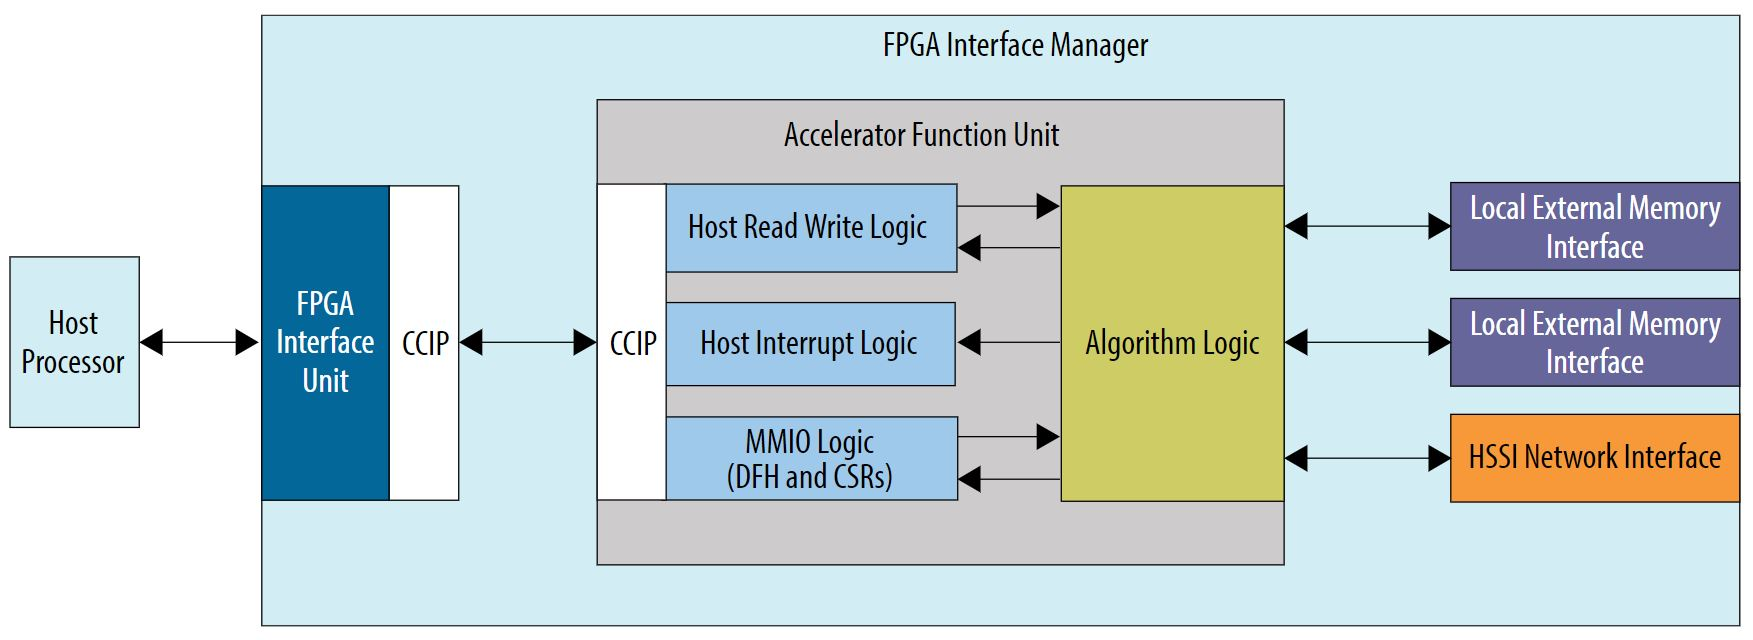
\includegraphics[scale=0.36]{figures/AFU.JPG}
     \caption{A block diagram of AFU}
     \label{fig:AFU}
 \end{figure}
 
\noindent 
The MMIO Logic of an AFU facilitates access to some {\it registers}. This circuitry provides address decoding that allows the processor to read/write AFU registers using memory-mapped I/O. Some of these registers have dedicated purposes that are required to be compatible with the Intel Acceleration Stack. Other registers are part of the {\it Application Logic} in the AFU, which is the part of the AFU that is used to perform computations along with the processor.\\

The Host Read Write Logic facilitates access to local FPGA memory and shared memory with the processor. This circuitry implements direct memory access that allows the FPGA to move large amounts of data to and from the processor's memory.


\subsection{Core Cache Interface Protocol}
For this tutorial, we will use the {\it Core Cache Interface} protocol\textsuperscript{\textregistered} (CCI-P) for the data transfers between the FIU and the AFU. The Intel Acceleration Stack provides an interface for CCI-P. The interface is composed of three request/response channels:
\begin{itemize}
    \item Channel 0 is used by the AFU for requests to read the processor's memory and responses. Channel 0’s response port is also used for receiving MMIO read and write requests from the processor.
    \item Channel 1 is used by the AFU for requests to write the processor's memory and responses.
    \item Channel 2 is used by the AFU for sending MMIO read responses back to the processor.
\end{itemize}
\noindent
To use the interface, we need to include the header file {\it platform\_if.vh} in the AFU source files. 


\subsection{Memory-Mapped I/O}
As shown in Figure \ref{fig:AFU}, an AFU has some logic for reading and writing registers. Figure \ref{fig:MMIO_code} provides an example AFU that contains the MMIO Logic. The AFU implements a 4-bit adder. The {\it Sum} register is set to the sum of {\it Num1} and {\it Num2}.\\


\noindent
The AFU module is required to have the name {\it afu}, as given in the figure. Depending on its functionality, an AFU may have different ports. For this example, in addition to {\it clock} and {\it reset} inputs, we require an input, called {\it rx}, and an output, called {\it tx}. The {\it rx} channel is used for receiving data and consists of the response ports of Channel 0 and 1 of the CCI-P interface. The {\it tx} channel is used for transmitting data and consists of the request ports of all three channels of the CCI-P interface.\\
\\
In Part a of Figure \ref{fig:MMIO_code}, the AFU receives a MMIO write request from the processor. Line \ref{line:h1} and \ref{line:h2} declare a special type of CCI-P signal called {\it mmioHdr}. This signal provides the {\it address} of the register currently being accessed by the processor, which is assigned to the 16-bit signal A in Line \ref{line:A}. The address is implemented in the CCI-P as an {\it offset} from a {\it base} address that is used for memory-mapped I/O. Each address is aligned to a double-word (32-bit) boundary in the processor's address space. When the processor is performing a write to a register in the AFU, the write control signal {\it W} will be 1 and the {\it data} signal {\it D} is valid.  \\
\\
The {\it always\_ff} block in Line \ref{line:reg} shows how the AFU can update a register during a processor's {\it write} command.\\
\\
In Part b of Figure \ref{fig:MMIO_code}, the AFU receives a read request from the host and send the response back to the host. The figure gives mandatory code that must be present in an AFU to support read operations from the processor at specific addresses. These addresses are decoded
in the AFU by using the {\it case} statement in Line~\ref{line:case}. As shown, each
address responds by placing data onto Channel 2's {\it tx} output of the AFU. For address $A = 0$
the AFU responds with a particular 64-bit data pattern that is required for any AFU, which is called {\it Device Feature Header} (DFH). Addresses
$A=2$ and $A=4$ respond with the low and high 64-bits of the {\it afu\_id} signal. This signal
represents a globally-unique identifier for the AFU. It is declared in Line~\ref{line:afu_id}
and initialized with the symbolic constant \texttt{AFU\_ACCEL\_UUID}, which is
defined in the file {\it afu\_json\_info.vh}.  Finally, addresses $A=6$ and $A=8$
respond with 0 for our AFU.\\
\\
In Part c, lines \ref{line:Num1} to \ref{line:Cout} allow the processor to read num1, num2, sum and carry-out bit at the addresses $A=(10)_{16}$, $A=(12)_{16}$, $A=(14)_{16}$ and $A=(16)_{16}$, respectively. As mentioned previously, each address $A$ represents a double-word (32 bit) processor address. This means that the addresses decoded in our case statement are aligned to a quad-word (64 bit) boundary, because the least-significant address bit $A_0 =0$ for each address. The CCI-P specification requires this alignment for all registers in an AFU.\\

\lstset{language=Verilog,morekeywords={enum,logic,always_ff, always_comb},numbers=left,escapechar=|}
\begin{figure}[h]
\begin{center}
\begin{minipage}[h]{16 cm}
\begin{lstlisting}[name=AFU]
|\label{line:platform}|`include "platform_if.vh"
|\label{line:json}|`include "afu_json_info.vh"

module afu (clock, reset, rx, tx);
    input  clock;                   // CCI-P clock
    input  reset;                   // CCI-P reset
    |\label{line:rx}|input  t_if_ccip_Rx rx;         // receive channel
    |\label{line:tx}|output t_if_ccip_Tx tx;         // transmit channel
    
    logic [15:0] A;                      // Address
    logic [31:0] D;                     // Data
    logic W;                          // Write signal
    logic [3:0] Num1;
    logic [3:0] Num2;
    logic [4:0] Sum;

    |\label{line:h1}|t_ccip_c0_ReqMmioHdr mmioHdr;   // channel c0 header
    |\label{line:h2}|assign mmioHdr = t_ccip_c0_ReqMmioHdr'(rx.c0.hdr);
    |\label{line:A}|assign A = mmioHdr.address;     // rename address signal
    assign D = rx.c0.data;          // rename data signal
    assign W = rx.c0.mmioWrValid;   // rename write signal
    |\label{line:reg}|always_ff @(posedge clock) begin
        if (reset) begin
            Num1 <= '0;
            Num2 <= '0;
        end
        else if (W) begin
            if(A == 16'h0010)
                Num1 <= D[3:0];
            else if (A == 16'h0012)
                Num2 <= D[3:0];
        end
    end

\end{lstlisting}
\end{minipage}
\caption{Adder AFU Verilog code (Part $a$).}
\label{fig:MMIO_code}
\end{center}
\end{figure}


\lstset{language=Verilog,morekeywords={enum,logic,always_ff},numbers=left,escapechar=|}
% \begin{figure}[h]
\begin{minipage}[h]{17 cm}
\begin{lstlisting}[name=AFU]
    always_comb
        if (reset)
            Sum = '0;
        else
            Sum = Num1 + Num2;
            
    |\label{line:afu_id}|logic [127:0] afu_id = `AFU_ACCEL_UUID; // from afu_json_info.vh

    always_ff @(posedge clock) begin // respond to memory-mapped I/O reads
        if (reset) begin
            tx.c1.hdr <= '0;
            tx.c1.valid <= '0;
            tx.c0.hdr <= '0;
            tx.c0.valid <= '0;
            tx.c2.hdr <= '0;
            tx.c2.mmioRdValid <= '0;
        end
        else begin
            // clear read response flag in case there was a response last cycle
            tx.c2.mmioRdValid <= 0;

            // serve MMIO read requests
            if (rx.c0.mmioRdValid == 1'b1) begin
                // copy TID, which host needs to map response to request
                tx.c2.hdr.tid <= mmioHdr.tid;
                // post response
                tx.c2.mmioRdValid <= 1;

                |\label{line:case}|case (A)
                    // AFU header
                    |\label{line:DFH}| 16'h0000: tx.c2.data <= {
                        4'b0001, // Feature type = AFU
                        8'b0,    // reserved
                        4'b0,    // afu minor revision = 0
                        7'b0,    // reserved
                        1'b1,    // end of DFH list = 1
                        24'b0,   // next DFH offset = 0
                        4'b0,    // afu major revision = 0
                        12'b0    // feature ID = 0
                    };
                    16'h0002: tx.c2.data <= afu_id[63:0];   // AFU_ID_L
                    16'h0004: tx.c2.data <= afu_id[127:64]; // AFU_ID_H
                    16'h0006: tx.c2.data <= 64'h0;          // DFH_RSVD0
                    16'h0008: tx.c2.data <= 64'h0;          // DFH_RSVD1
                    
\end{lstlisting}
\begin{center}
Figure 2. Adder AFU Verilog code (Part $b$).
\end{center}
\end{minipage}
% \end{figure}

\lstset{language=Verilog,morekeywords={enum,logic,always_ff},numbers=left,escapechar=|}
% \begin{figure}[h]
\begin{minipage}[h]{17 cm}
\begin{lstlisting}[name=AFU]
                    // application logic registers
                    |\label{line:Num1}|16'h0010: tx.c2.data <= 64'(Num1);
                    16'h0012: tx.c2.data <= 64'(Num2);
                    16'h0014: tx.c2.data <= 64'(Sum[3:0]);
                    |\label{line:Cout}|16'h0016: tx.c2.data <= 64'(Sum[4]);

                    default:  tx.c2.data <= 64'h0;
                endcase
            end
        end
    end
endmodule
\end{lstlisting}
\begin{center}
Figure 2. Adder AFU Verilog code (Part $c$).
\end{center}
\end{minipage}
% \end{figure}

~\\
\subsection{Platform Configuration}
For an AFU to use the framework provided by the FIM, we need to include the Platform Configuration for the AFU in a {\it JavaScript Object Notation} (JSON) file. The platform configuration file specifies the AFU's  {\it Universally Unique Identifier} (UUID), the {\it top-level interface} for the AFU to connect with the FIU and external interfaces to access local memory, network, etc. \\
\\
Figure \ref{fig:json} shows the platform configuration file for the AFU example. This file specifies the type of CCI-P port used for the AFU, which is called {\it ccip\_std\_afu}.  This interface consists of 
{\it clock}, {\it reset}, receive ({\it rx}) and transmit ({\it tx}) ports, as given 
in Figure~\ref{fig:MMIO_code}. The file also specifies the AFU name, {\it adder\_afu}, and its UUID. The UUID shown in the figure is just a placeholder. You need to generate a new UUID for the AFU by using the {\it uuidgen} command that is available on the DevCloud.

\lstset{language=Java,numbers=none,escapechar=|}
\begin{figure}[h]
\begin{center}
\begin{minipage}[h]{15 cm}
\begin{lstlisting}[name=json]
{
    "version": 1,
    "afu-image": {
        "power": 0,
        "afu-top-interface": {
            "class": "ccip_std_afu"
        },
        "accelerator-clusters": [
            {
                "name": "adder_afu",
                "total-contexts": 1,
                "accelerator-type-uuid": "850adcc2-6ceb-4b22-9722-d43375b61c66"
            }
        ]
    }
}
\end{lstlisting}
\end{minipage}
\vspace{-.5cm}
\caption{The JSON file.}
\label{fig:json}
\end{center}
\end{figure}

\subsection{Generating Accelerator Function (AF)}
An Accelerator Function (AF) is a compiled hardware accelerator implemented in an FPGA device. To build an AF from the Verilog code module, you need to perform the following steps:
\begin{enumerate}
\item
Make a new folder on your home computer called \texttt{adder\_afu}. Then, in this folder create two
subfolders named \texttt{hw} and \texttt{sw}. The \texttt{sw} folder will be used for the software application that uses the ADDER AFU. Now, in the \texttt{hw} folder make a subfolder called \texttt{rtl}. You should now have created the folders illustrated in Figure~\ref{fig:folders}. This arrangement of folders is required when using the compilation tools that are provided on the DevCloud.

\begin{figure}[h]
  \begin{center}
      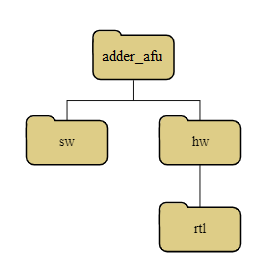
\includegraphics[]{figures/fig4.png}
  \end{center}
  \caption{The arrangement of folders for an AFU.}
	\label{fig:folders}
\end{figure}

\item
The code shown in Figure~\ref{fig:MMIO_code} is provided for you in the file {\it afu.sv} in folder \texttt{MMIO\_example/hw/} that is part of the {\it design\_files} material included along with this tutorial. Copy this file to the \texttt{rtl} folder you created in step 1.

\item
To compile the Verilog code for your AFU, the development tools on the DevCloud require several files in addition to {\it afu.sv}. The names of the required files have to be listed in a {\it plain-text} file named {\it filelist.txt} in the \texttt{rtl} folder. The contents of this file for our AFU is shown in Figure~\ref{fig:filelist}. The first file listed is the platform configuration file 
{\it adder\_afu.json}. The Verilog source-code files listed in {\it filelist.txt} specify the AFU and its CCI-P interface. The files {\it ccip\_interface\_reg.sv} and {\it ccip\_std\_afu.sv} have to be present in the AFU's 
\texttt{rtl} folder.

~\\
\noindent
The files {\it filelist.txt}, {\it adder\_afu.json}, {\it ccip\_interface\_reg.sv}, and 
{\it ccip\_std\_afu.sv} are also provided for you in \texttt{MMIO\_example/hw/}. Copy these files into your \texttt{rtl} folder, to
create the structure of files illustrated in Figure~\ref{fig:files}.

\lstset{language=C,numbers=none,escapechar=|}
\begin{figure}[h]
\begin{center}
\begin{minipage}[h]{4.5 cm}
\begin{lstlisting}[name=filelist]
adder_afu.json

afu.sv
ccip_interface_reg.sv
ccip_st_afu.sv
\end{lstlisting}
\end{minipage}
\caption{The contents of {\it filelist.txt}.}
\label{fig:filelist}
\end{center}
\end{figure}


\item
For the remainder of the steps we assume that you are able to login to the DevCloud
and configure the environment variables and settings that are needed for AFU development. 
To perform this step it is important to be familiar with the material presented in the
tutorial {\it Using the Intel FPGA DevCloud for AFU Development}. First, 
copy the folders and files shown in Figure~\ref{fig:files} onto the DevCloud.  Then, 
using the Linux command line interface on the DevCloud execute the command 
\texttt{uuidgen} to generate a new UUID for the MMIO AFU.
Enter this new UUID into the file {\it adder\_afu.json}, replacing the placeholder given in
Figure~\ref{fig:json}.

\item
On the DevCloud, set your working directory to the \texttt{adder\_afu} folder, and then 
run the command: 

\noindent
\begin{center}
\texttt{afu\_synth\_setup -s hw/rtl/filelist.txt build\_synth}
\end{center}

Now, change your working directory to the newly-created \texttt{build\_synth} folder and 
execute the command \texttt{run.sh}. This command uses the information in 
the {\it adder\_afu.json} file to generate the Verilog header file {\it afu\_json\_info.vh}, 
which is included in the code shown in Figure~\ref{fig:MMIO_code}. 
The \texttt{run.sh} command then executes the Intel 
Quartus\textsuperscript{\textregistered} Prime software to compile the AFU into a circuit
that can be implemented in the target FPGA device.

~\\
\noindent
The Quartus Prime software begins by executing its synthesis tools that
compile your Verilog source code. If any syntax errors are reported (they are shown in 
\red{red}), then fix these errors and compile again. Note that it is 
``normal'' to receive a significant number of warning messages from the Quartus Prime 
software when compiling an AFU; while you should still monitor these messages, those that
refer to code that is not part of your design files can usually be ignored.

~\\
\noindent
After successful compilation of your AFU code, the Quartus Prime software generates an FPGA 
programming bit-stream file called {\it adder\_afu.gbs}. In Intel\textsuperscript{\textregistered}
FPGA literature, this type of file is known as a {\it Green Bitstream} and represents a 
{\it partial-reconfiguration} file for the target FPGA. You can download this {\it gbs} file 
into the FPGA device on the DevCloud, where it joins the main bit-stream that is 
already present in the FPGA. Intel refers to the main bit-stream as the {\it Blue Bitstream}. 
To download your AFU into the FPGA execute the command:

\noindent
\begin{center}
\texttt{fpgasupdate adder\_afu.gbs}.
\end{center}

Note that if you are using version 1.2.1 of the Arria 10 Development Stack on the
DevCloud, then you have to execute two commands to program the FPGA. First, execute:

\noindent
\begin{center}
\texttt{PACSign PR -t UPDATE -H openssl\_manager -i adder\_afu.gbs -o adder\_afu\_unsigned.gbs}
\end{center}

\noindent Type \texttt{y} ({\it yes}) in answer to the queries that are issued by this command. 
Then, execute:

\noindent
\begin{center}
\texttt{fpgasupdate adder\_afu\_unsigned.gbs}.
\end{center}
\end{enumerate}

\begin{figure}[H]
  \begin{center}
      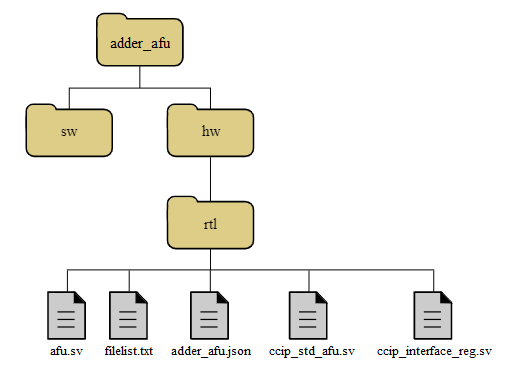
\includegraphics[scale=0.8]{figures/fig6.png}
  \end{center}
  \caption{The files needed for an AFU.}
	\label{fig:files}
\end{figure}


\noindent
Now that the AFU has been downloaded into the target FPGA device, we can develop software 
programs which run on the processor and make use of the AFU.

\section{Direct Memory Access (DMA)}
The processor only has access to an AFU's 256KB MMIO space. To move large workload of data to and from the processor's memory, we need to implement Direct Memory Access(DMA) in the AFU.
\subsection{DMA AFU}
The {\it dma\_afu} example shows how to manage memory transfers between the processor and the FPGA. The design files for this AFU can be found at \verb|$OPAE_PLATFORM_ROOT/hw/samples/dma_afu/hw/rtl/| on the DevCloud.\\
\\
Figure \ref{fig:DMA_AFU} provides the high level diagram of a Direct Memory Access (DMA) AFU. The data from the FIU is first separated into an MMIO channel, which transmits control and status data, and a DMA channel, which is used for moving larger blocks of data. The AFU uses Avalon-MM interface for its application logic circuit (DMA Test System), and thus a CCI-P to Avalon-MM Adapter is added to convert the CCI-P interface to the Avalon-MM interface. The DMA channel is further separated into a memory-mapped read channel and a memory-mapped write channel.
\begin{figure}[H]
    \begin{center}
        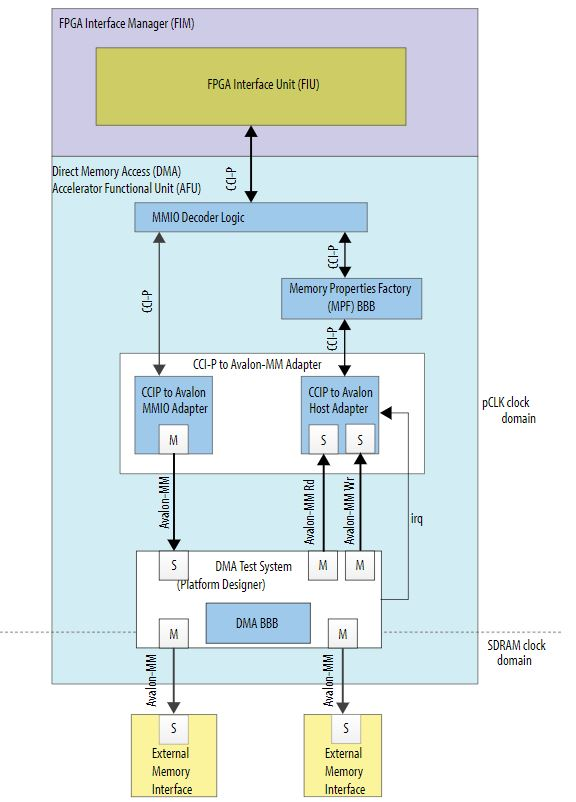
\includegraphics[width=0.55\textwidth]{figures/DMAAFU.JPG}
    \end{center}
    \caption{A block diagram of DMA AFU}
    \label{fig:DMA_AFU}
\end{figure}

\noindent
The code for the CCI-P to Avalon-MM Adapter is in folder \verb|BBB_ccip_avmm| and the modules are added to {\it afu.sv} to convert the signals. The Memory Properties Factory (MPF) ensures that read responses from the DMA return in the order that they were issued, which is required by the Avalon-MM protocol. The MMIO Decoder Logic separates MMIO reads and writes from the CCI-P RX channel. This ensures that the MMIO transfers never reaches the MPF. The MPF and the Decoder modules are added to the top-level file {\it ccip\_std\_afu.sv}.\\
\\
Figure \ref{fig:dmaSystem} shows the diagram for the DMA test system. The \texttt{AFU ID} component stores the mandatory information, including the 64-bit DFH and the UUID of the AFU, to support read operations from the processor at specific addresses. The DMA Basic Building Block (BBB) is used for data transfer between the processor and the FPGA's local memory.
\begin{figure}[H]
    \centering
    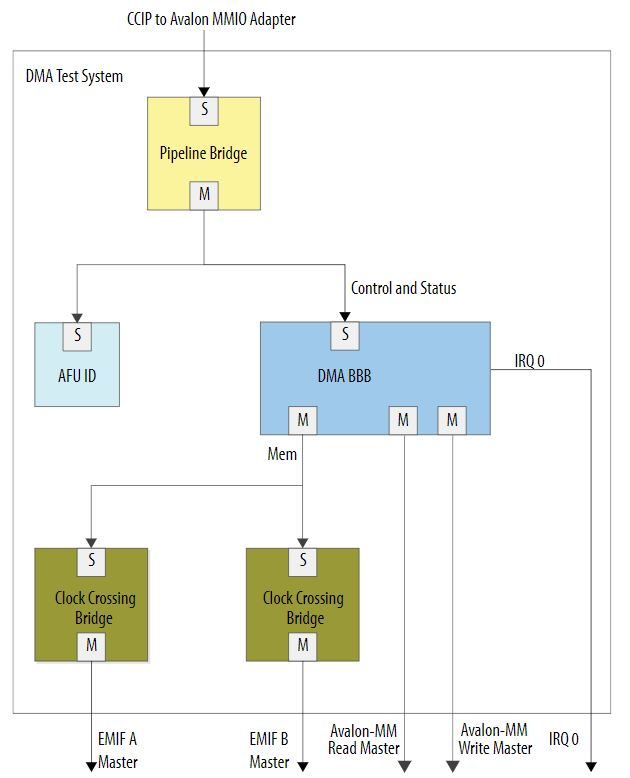
\includegraphics[width=0.55\textwidth]{figures/DMATestSystem.JPG}
    \caption{DMA System}
    \label{fig:dmaSystem}
\end{figure}

\noindent
Figure \ref{fig:dmaBBB} provides a more detailed view of the DMA BBB subsystem. The \texttt{BBB ID} component stores the DFH and UUID of the DMA BBB. The software application will use this component to identify the functionality of this subsystem. The subsystem receives MMIO read/write requests from the processor and sends responses back through the Control and Status (CSR) Pipeline Bridges. The Host Pipeline Bridges are connected to the Avalon-MM Rd and Wr ports of the CCI-P to Avalon-MM Adapter for DMA data transfers. The Memory Pipeline Bridge is connected the FPGA's local memory.\\


The DMA transfers are performed by the Modular Scatter-Gather DMA (MSGDMA). The MSGDMA transfers a cache line (64 bytes) per clock cycle. The data transferred by this component must be 64-byte aligned and the transfer length must be a multiple of 64 bytes. The Magic Number ROM is used for creating a barrier in the host (processor) memory during a DMA write. The Address Span Extender implements memory transfers that are not 64-byte aligned. It exposes a 4KB window of the local memory to the processor and the processor accesses the data window through MMIO.

\begin{figure}[H]
    \centering
    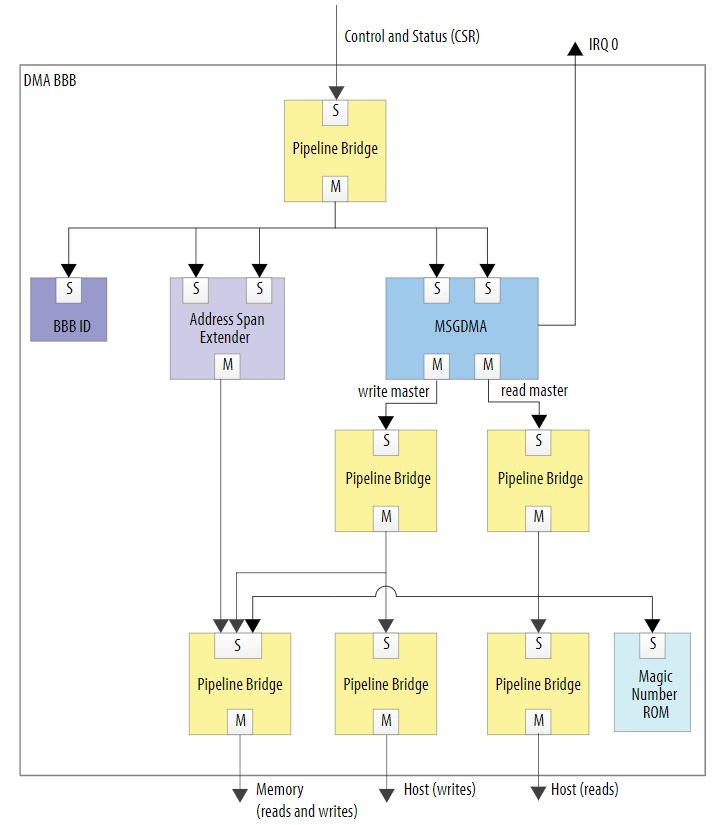
\includegraphics[width=0.6\textwidth]{figures/DMABBB.JPG}
    \caption{DMA BBB}
    \label{fig:dmaBBB}
\end{figure}

\subsection{Creating a DMA AFU}
You can expand the DMA AFU for your own application by adding hardware components to process local data and using the DMA AFU to move data between the host memory and the FPGA local memory. In this section, we will expand the sample DMA AFU with the {\it color\_converter} module in {\it design\_files} accompanying this tutorial.

\noindent
The {\it color\_converter} module converts an image in grayscale format, which is stored as an array of 8-bit pixel value (0-255) in the FPGA's local memory, to an image in RGB format (24-bit pixel value) and writes the result back to the local memory. It has an Avalon-MM master interface, named {\it m0}, and an Avalon-MM slave interface, named {\it s0}, apart from the {\it clk} and {\it reset} input ports. The master interface is used for accessing the local memory, so it needs to be connected to the Clock Crossing Bridges in Figure \ref{fig:dmaSystem}. The slave interface is used for receiving and responding to the control signals. For the module to be controlled by the processor, the slave interface needs to be connected to the Pipeline Bridge in Figure \ref{fig:dmaSystem}, the other end of which is the CCIP to Avalon MMIO Adapter.\\
\\
Figure \ref{fig:CSC_verilog} shows the Verilog code for the {\it color\_converter} interacting with signals from the {\it s0} interface. The {\it color\_converter} uses the {\it write} signals from {\it s0} as the command to process an image. When the {\it s0\_write} signal is 1 and the {\it s0\_address} signal is 0, the module considers the {\it s0\_writedata} as valid and will start converting an image. The module gets the size of the grayscale image from {\it s0\_writedata} and then converts it to the address to write the result image.  The DMA View in Figure \ref{fig:dmaMemView} shows the address space on the FPGA. The lowest two blocks of memory map to the two banks of the FPGA's DDR SDRAM. The {\it color\_converter} assumes that the source image will be stored starting at address {\it 0x0}, and it writes the result image right after the source image, which is at address {\it size\_of\_image}.

\lstset{language=Verilog,morekeywords={logic,always_ff},numbers=none,escapechar=|}
\begin{figure}[H]
\begin{center}
\begin{minipage}[h]{\textwidth}
\begin{lstlisting}[name=color_converter]
module color_converter(clk, reset, s0_write, s0_writedata, s0_address, s0_read, s0_readdata, readdata, readdatavalid, waitrequest, address, read, write, writedata);
    parameter NUM_BYTES = 64, n = 512;
    input clk, reset;
    input s0_write, s0_read, s0_address;
    input [63:0] s0_writedata;
    output logic [63:0] s0_readdata;
    input [n-1:0] readdata;
    input readdatavalid, waitrequest;
    output logic [47:0] address;
    output logic read, write;
    output logic [n-1:0] writedata;
    logic convert_done;
    logic [47:0] src_address, dst_address;
    
    always @(posedge clk) begin
        if(reset)
            s0_readdata <= '0;
        else if(s0_read)begin
            if(s0_address == 0) 
                s0_readdata <=  {16'h0, dst_address};
            else if(s0_address == 1)
                s0_readdata <= {63'h0, convert_done};
        end
    end
    
    always @(posedge clk) begin
        if(reset) begin
            src_address <= '0;
            dst_address <= '0;
        end
        else if(s0_write && s0_address == 0) begin
            src_address <= '0;
            dst_address <= s0_writedata[47:0];
        end
    end
        |$\ldots$| 
endmodule
\end{lstlisting}
\end{minipage}
\caption{Verilog code for {\it color\_converter} MMIO logic.}
\label{fig:CSC_verilog}
\end{center}
\end{figure}

\begin{figure}[h]
    \centering
    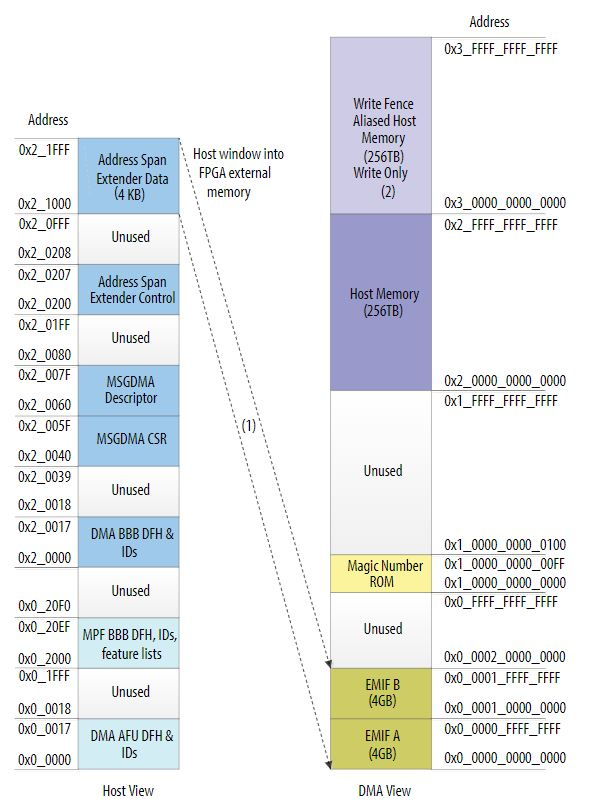
\includegraphics[width=0.5\textwidth]{figures/DMAMemView.JPG}
    \caption{AFU and Host Views of Memory}
    \label{fig:dmaMemView}
\end{figure}

\noindent
The {\it color\_converter} also keeps track of the status of a conversion in the register {\it convert\_done} and will set {\it s0\_readdata} port to the value of {\it convert\_done} upon a read request($s0\_read==1$ AND $s0\_address==1$) from the processor. If a conversion completes, the value will be 1, otherwise it will be 0. Since the control and status signals are transferred through MMIO, we need to specify an address space for the processor to read/write the registers in {\it color\_converter}. The Host View in Figure \ref{fig:dmaMemView} shows the processor's view of the address space in the sample design. The address space for the DMA system spans from 0x0\_0000 to 0x2\_1FFF. Some part of the address space has already been assigned to the other components in the DMA system. We will select an unused block of addresses for the color converter in the steps below.\\

\noindent
Perform the following steps to add {\it color\_converter} to the {\it DMA Test System}:
\begin{enumerate}
    \item Create a folder named \texttt{converter\_dma\_system} on your own computer and then copy the files in\\ \texttt{hw/rtl/qsys/A10/} of the \emph{dma\_afu} example from the DevCloud to the new folder. Also copy the\\ \texttt{DMA\_example/color\_converter} folder in {\it design\_files} for this tutorial to \texttt{converter\_dma\_system}. 
    \item In the \texttt{converter\_dma\_system} folder, create a new project named {\it dma\_test\_system} in Quartus. Select Arria 10 as the device family. Set {\it dma\_test\_system.qsys} as the top-level design. Ensure this file is not read-only.
    \item Open the {\it dma\_test\_system.qsys} in the Platform Designer. You may upgrade all ip cores if prompted. Instantiate the {\it color\_converter} in {\it dma\_test\_system.qsys} and make the following connections: 
        \begin{itemize}
            \item connect clock to host\_clk.out\_clk
            \item connect reset to reset\_in.out\_reset
            \item connect s0 to dma\_test\_system\_mm\_bridge\_0.m0
            \item connect m0 to ddr4\_mm\_bridge.s0
        \end{itemize}
    The resulting connections are shown in Figure \ref{fig:csc_connection}.
    \item Set the base address of {\it s0} of {\it color\_converter} to 0x0040, which is the first address available after the address space of the AFU ID component. 
    \item Click the \texttt{Generate HDL} button at bottom-right of the Platform Designer, and click \texttt{Generate} in the popup window. After this is completed, you may exit platform designer.
\end{enumerate}
\begin{figure}[H]
    \centering
    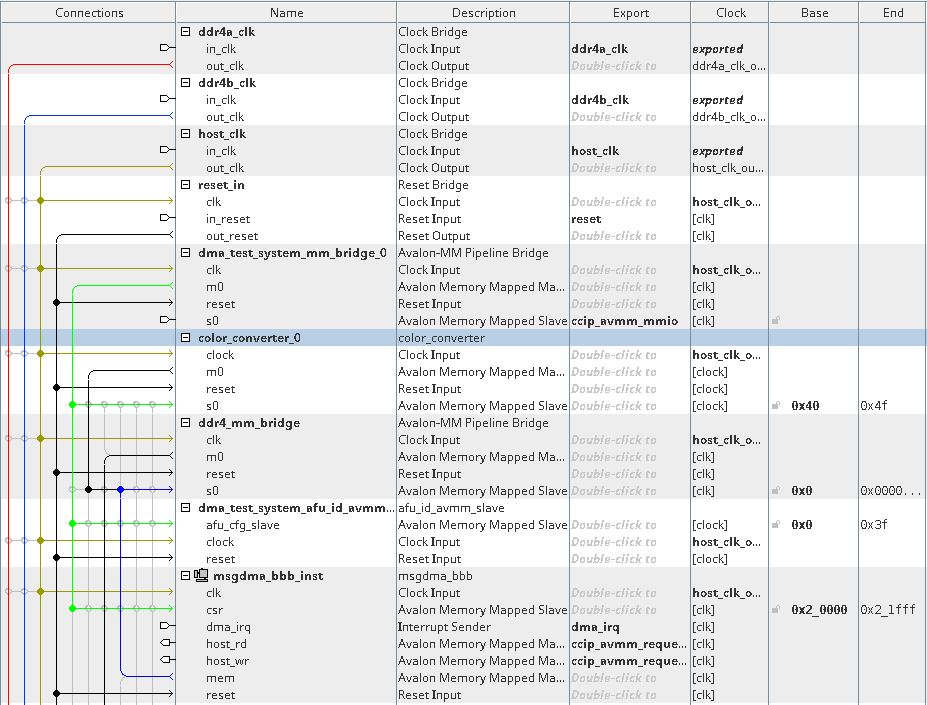
\includegraphics[width=0.8\textwidth]{figures/csc_ip_connection.JPG}
    \caption{color converter IP connection}
    \label{fig:csc_connection}
\end{figure}

\noindent
To generate an AF for the DMA AFU with color converter, perform the following steps on the DevCloud:
\begin{enumerate}
    \item Create a folder called \texttt{converter\_dma\_afu}. In \texttt{converter\_dma\_afu} create two subfolders named \texttt{hw} and \texttt{sw}. The \texttt{sw} subfolder will be used for the software application that uses this AFU. Copy the \texttt{hw/rtl/} folder of the {\it dma\_afu} example on DevCloud to the new folder. Next, replace the DMA Test System of the example with the system you created in {\it converter\_dma\_system}, i.e. copy the files in {\it converter\_dma\_system} from your computer to \texttt{converter\_dma\_afu/hw/rtl/qsys/A10/} and replace the files with the same names. Also copy the {\it color\_converter} folder and files to the A10 directory.
    
    \item Add the path to the design file ({\it .sv}) and the IP file ({\it .ip}) of {\it color\_converter}, as shown below,  to {\it filelist.txt} in \texttt{converter\_dma\_afu/hw/rtl/}. The paths are relative to the directory containing {\it filelist.txt}.
    
\lstset{language=C,numbers=none,escapechar=|}
\begin{lstlisting}[name=filelist]
qsys/A10/color_converter/color_converter.sv
qsys/A10/ip/dma_test_system/dma_test_system_color_converter_0.ip
\end{lstlisting}

    \item Use the Linux command line interface on the DevCloud execute the command 
\texttt{uuidgen} to generate a new UUID for the DMA AFU.
Enter this new UUID into the file {\it dma\_afu.json}, replacing the value of the key {\it accelerator-type-uuid}. Note that we use {\it ccip\_std\_afu\_avalon\_mm} as the `class' of {\it afu-top-interface}. {\it avalon\_mm} specifies the interface to the local FPGA memory.\\
\\
Around line 465, update the parameter {\it AFU\_ID\_H}  and {\it AFU\_ID\_L} of {\it dma\_test\_system\_afu\_id\_avmm\_slave\_0.ip} to the upper 16 digits and lower 16 digits of the new UUID, removing the dashes. The file is in\\ \texttt{hw/rtl/qsys/A10/ip/dma\_test\_system/}.

    \item  On the DevCloud, set your working directory to the \texttt{converter\_dma\_afu} folder, and then run the command: 

\noindent
\begin{center}
\texttt{afu\_synth\_setup -s hw/rtl/filelist.txt build\_synth}
\end{center}

Now, change your working directory to the newly-created \texttt{build\_synth} folder and 
execute the command \texttt{run.sh}. 
The \texttt{run.sh} command then executes the Intel 
Quartus\textsuperscript{\textregistered} Prime software to compile the AFU into a circuit
that can be implemented in the target FPGA device.

~\\
\noindent
The Quartus Prime software begins by executing its synthesis tools that
compile your Verilog source code. If any syntax errors are reported (they are shown in 
\red{red}), then fix these errors and compile again. 

~\\
\noindent
After successful compilation of your AFU code, the Quartus Prime software generates an FPGA 
programming bit-stream file called {\it dma\_afu.gbs}. You can download this {\it gbs} file into the FPGA device on the DevCloud by executing the command:

\noindent
\begin{center}
\texttt{fpgasupdate dma\_afu.gbs}.
\end{center}

Note that if you are using version 1.2.1 of the Arria 10 Development Stack on the
DevCloud, then you have to execute two commands to program the FPGA. First, execute:

\noindent
\begin{center}
\texttt{PACSign PR -t UPDATE -H openssl\_manager -i dma\_afu.gbs -o dma\_afu\_unsigned.gbs}
\end{center}

\noindent Type \texttt{y} ({\it yes}) in answer to the queries that are issued by this command. 
Then, execute:

\noindent
\begin{center}
\texttt{fpgasupdate dma\_afu\_unsigned.gbs}.
\end{center}

\end{enumerate}



\subsection{Streaming DMA AFU}
The {\it streaming\_dma\_afu} shows how to transfer data between the memory and Avalon-ST sources and sinks. The design files for this AFU can be found at\\ \verb|$OPAE_PLATFORM_ROOT/hw/samples/streaming_dma_afu/hw/rtl/| on the DevCloud.\\
\\
Similar to the DMA AFU example, the Streaming DMA AFU first separates MMIO and the DMA read and write channels. The MMIO channel is used for accessing control registers and the DMA read and write channels are used for transferring data the processor and the AFU. The AFU then converts the CCI-P interface to Avalon-MM interface for the DMA system.\\
\\
Figure \ref{fig:stSystem} illustrates the Streaming DMA Test System. The Memory-to-Stream (M2S) DMA BBB subsystem reads data from a buffer stored in memory (either the FPGA's local memory or shared memory with the processor) and converts it into an Avalon-ST source stream. The Stream-to-Memory (S2M) DMA BBB accepts a serial stream of data from its Avalon-ST sink port and writes the data to buffers in memory. In this example, the output stream from the M2S DMA BBB is sent to the Pattern Checker, and the input stream of the S2M DMA BBB comes from the Pattern Generator.\\

\begin{figure}[H]
    \centering
    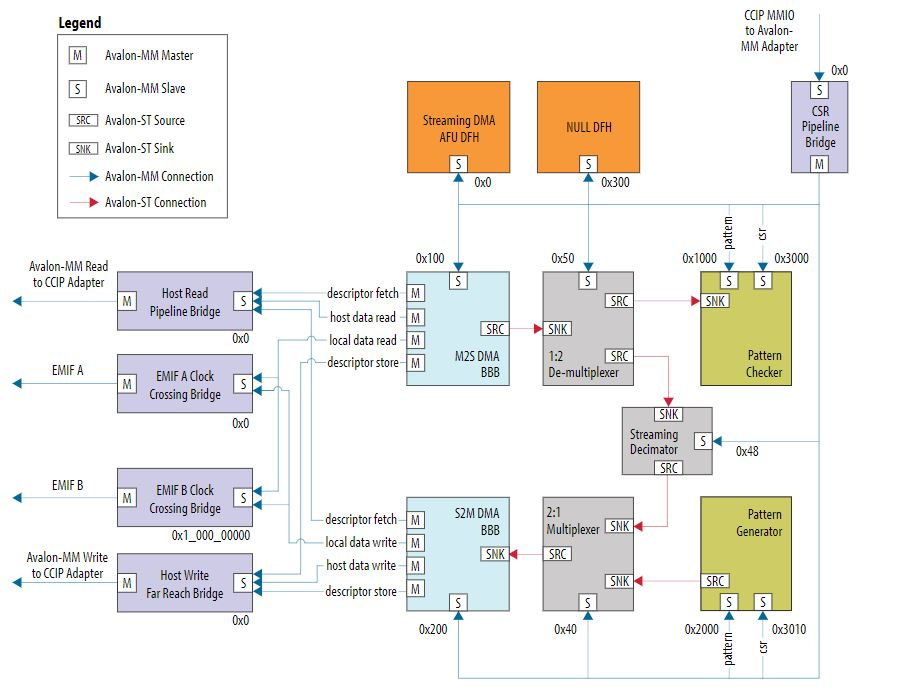
\includegraphics[width=0.70\textwidth]{figures/STSystem.JPG}
    \caption{Streaming DMA Test System}
    \label{fig:stSystem}
\end{figure}

\noindent
The AFU DFH component stores the 64-bit DFH and the UUID of the AFU.  Each of the M2S and S2M DMA BBBs also has a DFH for the processor to manage the DMA channels. As shown in Line \ref{line:DFH} in Figure \ref{fig:MMIO_code}, each DFH stores a ``pointer" (address offset) to the next DFH. The Null DFH component exposes the end of the DFH list outside of the DMA BBBs. It allows you to add more DMA logic to the design without modifying the DFH in the subsystems.

\subsection{Creating a Streaming DMA AFU}
You can adapt the streaming DMA AFU example for your own application. In this section, we will create an AFU that converts an image from grayscale format to RGBA format based on the {\it streaming\_dma\_afu} example. \\

\begin{figure}[h]
    \centering
    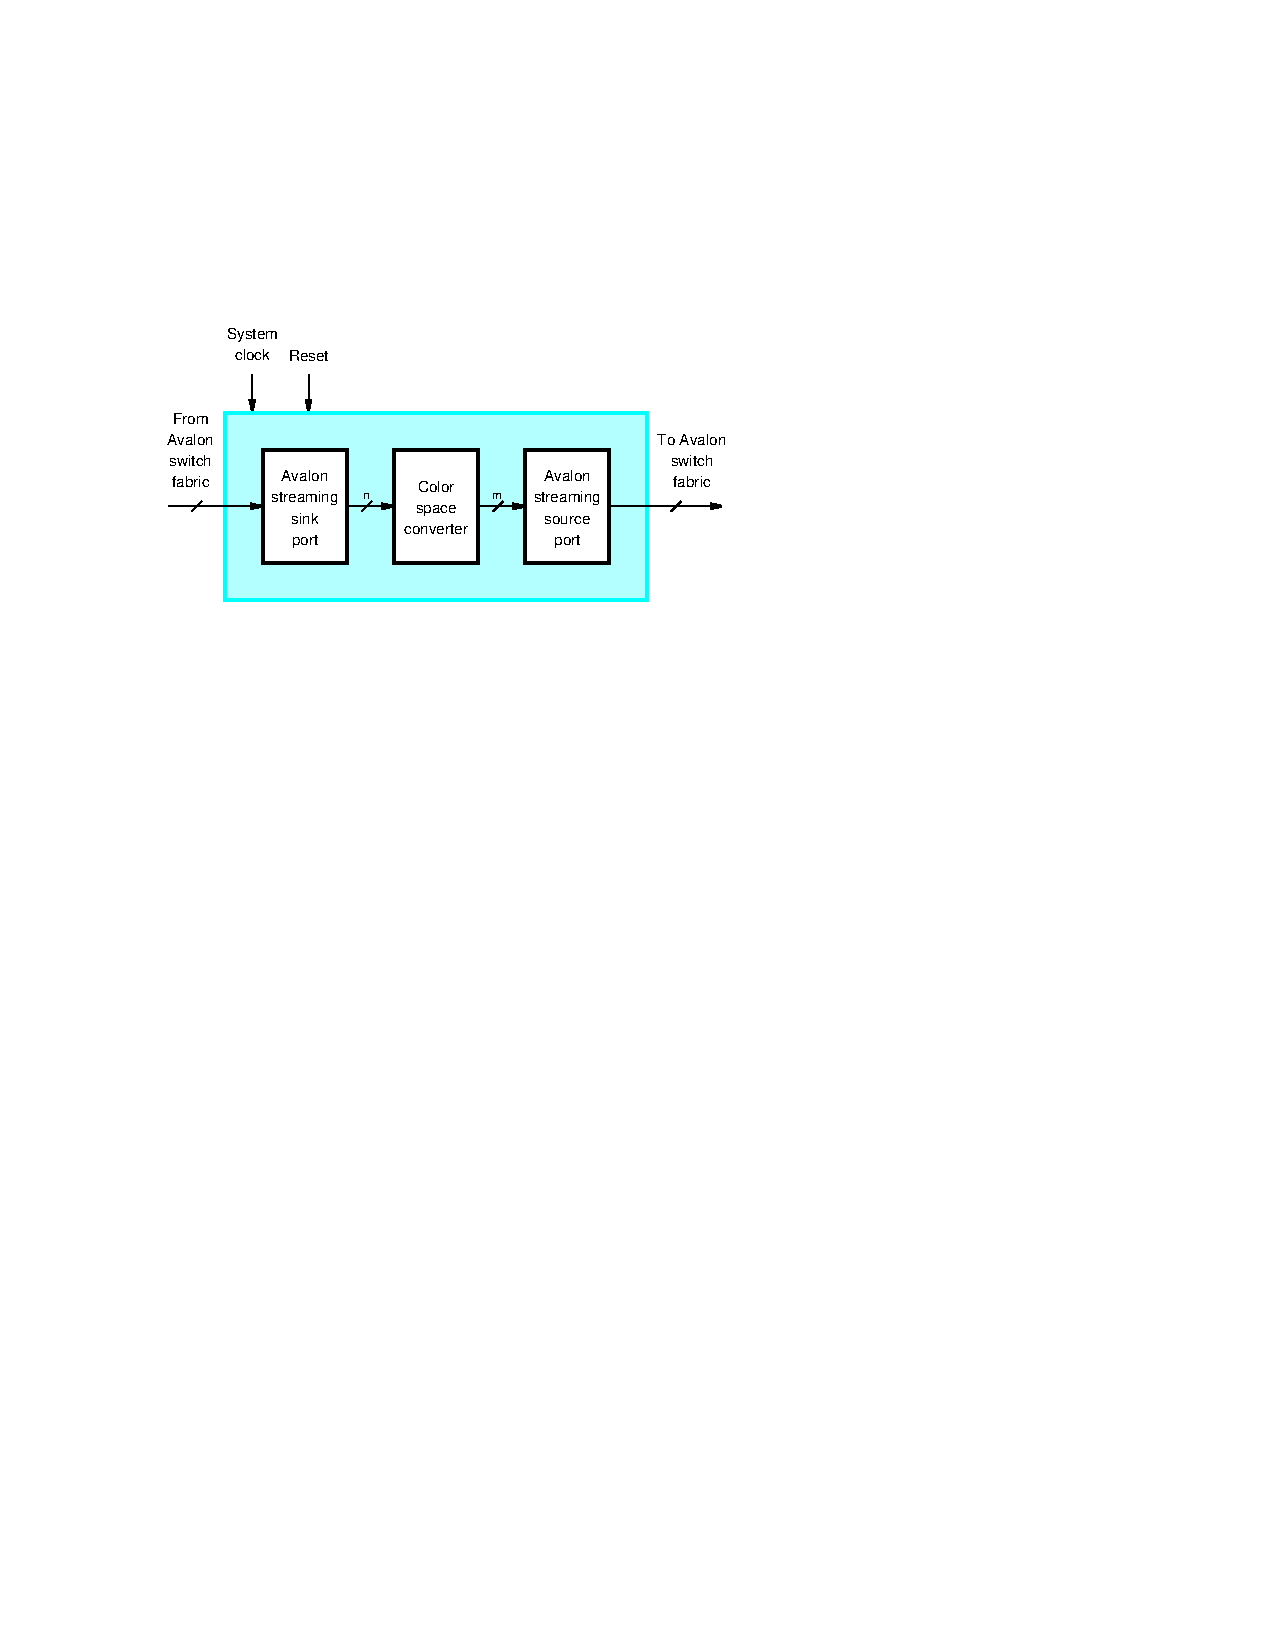
\includegraphics{figures/rgb_resampler.pdf}
    \caption{RGB Resampler core's block diagram.}
    \label{fig:resampler}
\end{figure}

\noindent
The RGB Resampler converts images between different RGB formats. Figure \ref{fig:resampler} shows a block diagram of the RGB Resampler. It accepts streaming data with an Avalon-ST sink port, then processes the data and passes the output to an Avalon-ST source port. We can replace the Pattern Checker and Generator in the Streaming DMA Test System with the RGB Resampler and connect the resampler between the M2S DMA BBB, which will provide the source image as a serial stream, and the S2M DMA BBB, which will send the result image back to the processor. The steps are as follows:\\
\begin{enumerate}
    \item A basic streaming DMA AFU is created from the example streaming DMA AFU with the application logic components (Pattern Checker and Generator, De-multiplexer, Multiplexer and Streaming Decimator) in the Streaming DMA Test System removed. You can find the basic streaming DMA AFU in the\\ \texttt{Streaming\_DMA\_example/hw/rtl} folder in {\it design\_files} included along with this tutorial. 
    
    \item Change your working directory to \texttt{Streaming\_DMA\_example/hw/rtl}. In the \texttt{TEST\_streaming\_dma} folder, create a Quartus project called \emph{streaming\_dma\_test\_system}. Select Arria 10 as the device family. Set \emph{streaming\_dma\_test\_system.qsys} as the top-level design. Ensure this file is not read-only.
    
    \item Open \emph{streaming\_dma\_test\_system.qsys} in the Platform Designer. You may upgrade all ip cores if prompted. In \texttt{IP Catalog} , expand \texttt{Library} $\rightarrow$ \texttt{University Program} $\rightarrow$ \texttt{Audio \& Video} $\rightarrow$ \texttt{Video}, click on \texttt{RGB Resampler Intel FPGA IP} and click Add to create an instance of the \texttt{RGB Resampler} IP core in the \emph{streaming\_dma\_test\_system}. Set the \texttt{Incoming Format} parameter to \texttt{8-bit Grayscale} and the \texttt{Outgoing Format} parameter to \texttt{32-bit RGBA}.\\
    \\
    Make the following connections for the RGB Resampler:
     \begin{itemize}
            \item connect clk to dma\_clk.out\_clk
            \item connect reset to reset\_in.out\_reset
            \item connect avalon\_rgb\_sink to m2s\_dma\_bbb.m2s\_st\_source
            \item connect avalon\_rgb\_source to s2m\_dma\_bbb.s2m\_st\_sink
        \end{itemize}
        The resulting connections are shown in Figure \ref{fig:st_connection}.
        
    \item Click \texttt{Generate} $\rightarrow$ \texttt{Generate HDL}, and click generate in the resulting popup window. After this is completed, you may exit platform designer.
\end{enumerate}

\begin{figure}[h]
    \centering
    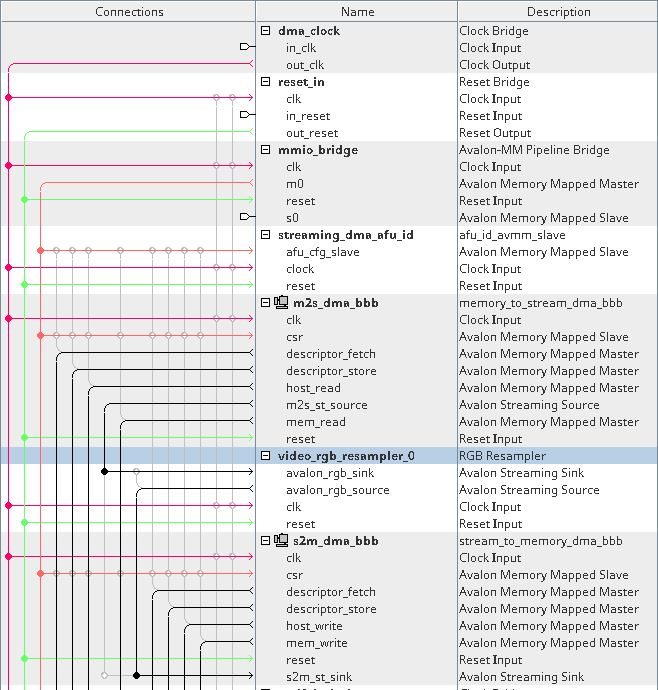
\includegraphics[width=0.75\textwidth]{figures/st_ip_connection.JPG}
    \caption{RGB Resampler IP interface connection}
    \label{fig:st_connection}
\end{figure}

~\\
\noindent
To generate an AF for this AFU, perform the following steps:
\begin{enumerate}
    \item In \texttt{Streaming\_DMA\_example/hw/rtl}, add the path to the IP file of the RGB Resampler to {\it filelist.txt}. The path is relative to the directory containing {\it filelist.txt}:
    
\lstset{language=C,numbers=none,escapechar=|}
\begin{lstlisting}[name=filelist]
TEST_streaming_dma/ip/streaming_dma_test_system/streaming_dma_test_system
_video_rgb_resampler_0.ip
\end{lstlisting}

    \item The following steps need to be done on the DevCloud. First, copy the \texttt{Streaming\_DMA\_example} folder and its subfolders onto the DevCloud. Then, using Linux command line interface on the DevCloud execute the command \texttt{uuidgen} to generate a new UUID for the AFU. Enter this new UUID into the file {\it streaming\_dma\_afu.json}, replacing the value of the key {\it accelerator-type-uuid}.
    
    Around line 465, update the parameter {\it AFU\_ID\_H} and {\it AFU\_ID\_L} of {\it streaming\_dma\_afu\_id.ip} to the upper 16 digits and lower 16 digits of the new UUID, removing the dashes. The IP file is in
    \begin{center}
    \texttt{TEST\_streaming\_dma/ip/streaming\_dma\_test\_system}.
    \end{center}
    
    \item  On the DevCloud, set your working directory to the \texttt{Streaming\_DMA\_example} folder, and then run the command: 

\noindent
\begin{center}
\texttt{afu\_synth\_setup -s hw/rtl/filelist.txt build\_synth}
\end{center}

Now, change your working directory to the newly-created \texttt{build\_synth} folder and 
execute the command \texttt{run.sh}. 
The \texttt{run.sh} command then executes the Intel 
Quartus\textsuperscript{\textregistered} Prime software to compile the AFU into a circuit
that can be implemented in the target FPGA device.

~\\
\noindent
The Quartus Prime software begins by executing its synthesis tools that
compile your Verilog source code. If any syntax errors are reported (they are shown in 
\red{red}), then fix these errors and compile again. 

~\\
\noindent
After successful compilation of your AFU code, the Quartus Prime software generates an FPGA 
programming bit-stream file called {\it streaming\_dma\_afu.gbs}. You can download this {\it gbs} file into the FPGA device on the DevCloud by executing the command:

\noindent
\begin{center}
\texttt{fpgasupdate streaming\_dma\_afu.gbs}.
\end{center}

Note that if you are using version 1.2.1 of the Arria 10 Development Stack on the
DevCloud, then you have to execute two commands to program the FPGA. First, execute:

\noindent
\begin{center}
\texttt{PACSign PR -t UPDATE -H openssl\_manager -i streaming\_dma\_afu.gbs -o streaming\_dma\_afu\_unsigned.gbs}
\end{center}

\noindent Type \texttt{y} ({\it yes}) in answer to the queries that are issued by this command. 
Then, execute:

\noindent
\begin{center}
\texttt{fpgasupdate streaming\_dma\_afu\_unsigned.gbs}.
\end{center}
 \end{enumerate}
 
 
 \section{Writing a Software Application}
 For the development of software, the OPAE SDK provides a library implementing the C API for discovering, accessing and managing FPGA devices and AFUs. We will write C programs with this library to utilize the adder AFU, color converter DMA AFU and streaming DMA AFU in previous parts.
 
 \subsection{MMIO}
 Figure \ref{fig:adder_code} shows a program that accesses the MMIO AFU in Section 2. This code includes the OPAE header file {\it mmio.h}, which provides the functions for memory-mapped I/O.\\
 
 \lstset{language=C,numbers=left,escapechar=|}
\begin{figure}[H]
\begin{center}
\begin{minipage}[h]{15 cm}
\begin{lstlisting}[name=C_code]
#include <stdio.h>
#include <stdlib.h>
#include <opae/mmio.h>
|\label{line:C_num1_reg}|#define NUM1_REG    0X10 << 2       // Application Logic
|\label{line:C_num2_reg}|#define NUM2_REG    0X12 << 2       // register addresses
|\label{line:C_sum_reg}|#define SUM_REG     0X14 << 2       // (offsets)
|\label{line:C_cout_reg}|#define COUT_REG    0X16 << 2       // 
|\label{line:open_AFU}|int open_AFU (fpga_handle *);
|\label{line:close_AFU}|void close_AFU (fpga_handle);

int main(int argc, char *argv[])
{
    if(argc < 3){
        printf("Usage: ./adder num1 num2\n");
        return -1;
    }
    |\label{line:C_AFU_handle}|fpga_handle handle = NULL;
    if (open_AFU (&handle) < 0)
        return -1;

    uint32_t num1, num2, sum, cout;
    num1 = atoi(argv[1]);
    num2 = atoi(argv[2]);

    (void) fpgaWriteMMIO32 (handle, 0, NUM1_REG, num1);   // set num1
    (void) fpgaWriteMMIO32 (handle, 0, NUM2_REG, num2);  // set num2
    (void) fpgaReadMMIO32 (handle, 0, SUM_REG, &sum);
    (void) fpgaReadMMIO32 (handle, 0, COUT_REG, &cout);
    printf ("Sum: %x, Carry-out: %x\n", sum, cout);

    close_AFU (handle);
    return 0;
}
\end{lstlisting}
\end{minipage}
\caption{Using the ADDER AFU in a C program.}
\label{fig:adder_code}
\end{center}
\end{figure}
 
 
 \noindent
 Line \ref{line:C_num1_reg} to Line \ref{line:C_cout_reg} in Figure \ref{fig:adder_code} define the addresses that software has to use to access the num1, num2, sum, and carry-out registers in the AFU. These addresses are the same as the ones given in Figure \ref{fig:MMIO_code}, except that they are shifted left by two bits. This bit-shifting converts the double-word(32-bit aligned) addresses used in the Verilog code to the byte addresses that are issued by the processor.\\
 \\
In Lines~\ref{line:open_AFU} and~\ref{line:close_AFU} prototypes are given for the functions {\it open\_AFU} and {\it close\_AFU}. The first of these functions sets up a communication mechanism between the software program and the AFU, via a Linux device driver. The second function terminates this connection. The {\it open\_AFU} function calls several OPAE library utilities to check if the AFU is available and working properly. If so, the {\it handle} variable, declared with the OPAE type {\it fpga\_handle} in Line~\ref{line:C_AFU_handle}, is set up as a {\it pointer} to the AFU. The {\it open\_AFU} function uses this pointer to ``print'' to the Linux Terminal the contents of the mandatory register addresses in the AFU, which are specified in Figure~\ref{fig:MMIO_code}. Appendix~A shows the source code for {\it open\_AFU}, in Figure~\ref{fig:open_AFU}. If it is able to communicate successfully with the AFU then the function returns 0, otherwise it returns -1. Figure \ref{fig:print} in Appendix A displays the code for the function {\it print\_AFU\_regs}, which is called by {\it open\_AFU}, and the code for {\it close\_AFU} is given in Figure~\ref{fig:close}.\\
\\
The remainder of the code uses memory-mapped I/O via the {\it handle} variable to access the registers in the ADDER AFU. The {\it fpgaReadMMIO32} function allows the software to read the contents of an AFU register, whereas {\it fpgaWriteMMIO32} allows a new value to be written to a register. The software code writes {\it num1} and {\it num2} to the AFU and then reads their sum and the carry-out bit.\\
\\
To run this program perform the following steps:
\begin{enumerate}
    \item Copy the files {\it adder.c} that contains the code in Figure \ref{fig:adder_code}, and a file named {\it manage\_afu.c}, which holds the C code for {\it open\_AFU} and {\it close\_AFU}, to the \texttt{sw} folder for the ADDER AFU on the DevCloud. The files are in the \texttt{MMIO\_example/sw} folder in {\it design\_files} for this tutorial.
    \item To compile the code in {\it adder.c} and {\it manage\_AFU.c} you have to use a special {\it Makefile} that employs the OPAE infrastructure on the DevCloud. Copy this {\it Makefile}, which is also included in the \texttt{MMIO\_example/sw}, into your \texttt{sw} folder. 
    \item In the \texttt{sw} directory on the DevCloud run the command \texttt{make}. The results are displayed in Figure~\ref{fig:adder_output}. As shown in the figure, one of the programs executed by \texttt{make} is {\it afu\_json\_mgr}. This program reads the file {\it adder\_afu.json} shown in Figure~\ref{fig:json} to find the UUID for the AFU, and then produces the C header file {\it afu\_json\_info.h}. This header file is used by {\it manage\_afu.c}. To execute your program you must first, as before, create the build\_synth directory, compile with \texttt{run.sh}, and update the fpga. Then type
    \texttt{./adder [num1] [num2]}, as illustrated in Figure~\ref{fig:adder_output}.
\end{enumerate}

\lstset{language=C,morekeywords={u42132@s005-n005,LFSR},numbers=none,escapechar=|}
\begin{figure}[H]
\begin{center}
\begin{minipage}[h]{\textwidth}
\begin{lstlisting}[name=output]
|\green{userid@s005-n005}:\blue{~/adder\_afu/sw}|$ ls
adder.c Makefile  manage_afu.c manage_afu.o
|\green{userid@s005-n005}:\blue{~/adder\_afu/sw}|$ make
afu_json_mgr json-info --afu-json=../hw/rtl/adder_afu.json --c-hdr=afu_json_info.h
Writing afu_json_info.h
gcc -fstack-protector -fPIE -fPIC -O2 -D_FORTIFY_SOURCE=2 -Wformat -Wformat-security -Werror -g -O2 -std=c99 -Wall -Wno-unknown-pragmas -c -o adder.o adder.c
gcc -fstack-protector -fPIE -fPIC -O2 -D_FORTIFY_SOURCE=2 -Wformat -Wformat-security -Werror -g -O2 -std=c99 -Wall -Wno-unknown-pragmas -c -o manage_afu.o manage_afu.c
gcc -fstack-protector -fPIE -fPIC -O2 -D_FORTIFY_SOURCE=2 -Wformat -Wformat-security -Werror -g -O2 -std=c99 -Wall -Wno-unknown-pragmas -o adder adder.o manage_afu.o -z noexecstack -z relro -z now -pie -luuid -lpthread -lopae-c
|\green{userid@s005-n005}:\blue{~/adder\_afu/sw}|$ ls
adder  adder.c  adder.o  afu_json_info.h  Makefile  manage_afu.c  manage_afu.o
|\green{userid@s005-n005}:\blue{~/adder\_afu/sw}|$ ./adder 1 2
Opening adder_afu
AFU DFH REG  = 0x1000010000000000
AFU ID HI    = 0x8becf8c725cb4457
AFU ID LO    = 0xbb7c61d00acfe6c2
AFU NEXT     = 0x0000000000000000
AFU RESERVED = 0x0000000000000000
Sum: 3, Carry-out: 0
|\green{userid@s005-n005}:\blue{~/adder\_afu/sw}||\$|./adder 9 10
Opening adder_afu
AFU DFH REG  = 0x1000010000000000
AFU ID HI    = 0x8becf8c725cb4457
AFU ID LO    = 0xbb7c61d00acfe6c2
AFU NEXT     = 0x0000000000000000
AFU RESERVED = 0x0000000000000000
Sum: 3, Carry-out: 1
\end{lstlisting}
\end{minipage}
\caption{Compiling and executing {\it adder.c}.}
\label{fig:adder_output}
\end{center}
\end{figure}




 
 \subsection{DMA}
 Figure \ref{fig:dma_C_code} shows a program that converts an image from grayscale format to RGB format using the DMA AFU with color converter. The code includes the header file \emph{fpga\_dma.h} which provides the API for setting up communication with the DMA BBB and controlling the DMA BBB to perform data transfers.\\
 \lstset{language=C,numbers=left}
\begin{figure}[H]
\begin{center}
\begin{minipage}[h]{17 cm}
\begin{lstlisting}[name=DMA_code, escapechar=\^]
#define CTRL_REG 0x40
#define STAT_REG 0x48

int main(int argc, char *argv[]){
	fpga_result res = FPGA_OK;
	fpga_dma_handle dma_h;
	fpga_handle afc_h;
	uint64_t *dma_buf_ptr = NULL;

	if(open_AFU(&afc_h) < 0)
		return -1;
		
	^\label{line:dma_open}^res = fpgaDmaOpen(afc_h, &dma_h);
	if(res != FPGA_OK || !dma_h)
		return -1;

	unsigned char * data, header;
	int width, height;
	if (read_grayscale(argv[1], &header, &data, &width, &height) < 0) 
		return -1;
	
	uint64_t count = width * height;
	^\label{line:dma_buf}^dma_buf_ptr = (uint64_t *)malloc_aligned(getpagesize(), count*3);
	if (!dma_buf_ptr)
		return -1;
	fill_buffer((char *)dma_buf_ptr, data, count);
	// copy from host to fpga
	^\label{line:dma_htom}^res = fpgaDmaTransferSync(dma_h, 0x0 /*dst */,
				  (uint64_t)dma_buf_ptr /*src */, count, HOST_TO_FPGA_MM);
	if(res != FPGA_OK)
		return -1;
	clear_buffer((char *)dma_buf_ptr, count);
	
	uint64_t control = count;
	res = fpgaWriteMMIO64 (afc_h, 0, CTRL_REG, control); 

	uint64_t converter_status = 0;
	while(converter_status != 1){
		res = fpgaReadMMIO64(afc_h, 0, STAT_REG, &converter_status);
	}

	// copy from fpga to host
	^\label{line:dma_mtoh}^res = fpgaDmaTransferSync(dma_h, (uint64_t)dma_buf_ptr /*dst */,
				  count /*src */, count*3, FPGA_TO_HOST_MM);
	if(res != FPGA_OK)
		return -1;

	write_result((char *)dma_buf_ptr, header, width, height);
}
\end{lstlisting}
\end{minipage}
\caption{Using the DMA AFU in a C program Part (a)}
\label{fig:dma_C_code}
\end{center}
\end{figure}

\lstset{language=C,numbers=left}
\begin{center}
\begin{minipage}[h]{17 cm}
\begin{lstlisting}[name=DMA_code]
	if (dma_buf_ptr)
		free_aligned(dma_buf_ptr);
	if (dma_h)
		res = fpgaDmaClose(dma_h);

	close_AFU(afc_h);
	return 0;
}
\end{lstlisting}
\begin{center}
Figure 18: Using the DMA AFU in a C program (Part b)
\end{center}
\end{minipage}
\end{center}
 The program first calls the \emph{open\_AFU} to set up a communication mechanism between the software program and the AFU. The code for this function is shown in Figure \ref{fig:open_AFU} in Appendix A. \\
 \\
 In Line \ref{line:dma_open}, the \emph{fpgaDMAOpen} function sets up additional environment for the direct memory access. The function first searches for the DFH of the DMA BBB in the opened AFU. If the DMA BBB is in the AFU, the function calls \emph{fpgaPrepareBuffer} to allocate page-aligned memory for shared access between the AFU and the software program. Then, it initializes a handle \emph{dma\_h} to the DMA BBB. If all steps are done successfully, it returns \texttt{FPGA\_OK}, otherwise it returns an error code. \\
 \\
The code then creates a buffer and makes a copy the image to process in the buffer. The buffer is allocated to a page-size aligned address because during data transfers, it will be mapped to the buffers in the shared memory, which are required to be page-aligned.\\
 \\
 In Line \ref{line:dma_htom} and \ref{line:dma_mtoh}, the code transfers the source image to the FPGA's local memory and transfers the result image back to the processor by calling the function \emph{fpgaDMATransferSync}. The function performs a transfer between a source address and a destination address. It controls the components in the DMA BBB in Figure \ref{fig:dmaBBB} via the \emph{dma\_h} variable to move data between the FPGA's local memory and the shared memory. The pointer to the buffer allocated in Line \ref{line:dma_buf} is used as the \emph{src} address for the host-to-FPGA transfer and also the \emph{dst} address for the FPGA-to-host transfer. The \emph{dst} address of the host-to-FPGA transfer is set to 0x0, which is the \emph{src\_address} defined by the \emph{color\_converter} IP to read the source image. The \emph{src} address of the FPGA-to-host transfer is set to the size of the image, which is the \emph{dst\_address} defined by \emph{color\_converter} to write the result image, as in Figure \ref{fig:CSC_verilog}. The \emph{fpgaDMATransferSync} function is a blocking call and returns a \emph{fpga\_result} when the transfer completes. \\
 \\
 After transferring the source image to the FPGA, the code writes the image's size to the \emph{color\_converter} through MMIO. The address \emph{CTRL\_REG}, defined in Line 1, is the base address we chose for \emph{s0} of the \emph{color\_converter} IP as shown in Figure \ref{fig:csc_connection}. The code then keeps checking the status of the conversion from the \emph{color\_converter} through MMIO until the conversion is completed. The address \emph{STAT\_REG}, defined in Line 2, corresponds to the address offset 1 in the \emph{color\_converter} IP.\\



\noindent
To run this program perform the following steps:
\begin{enumerate}
    \item Copy the files in \texttt{DMA\_example/sw} in \emph{design\_files} included along with this tutorial to the \texttt{sw} folder for the DMA AFU on the DevCloud. The file \emph{fpga\_dma\_test.c} contains the code shown in Figure \ref{fig:dma_C_code}. \emph{image\_helper.c} provides helper functions to read and write BMP images. \emph{manage\_afu.c} holds the code for \emph{open\_AFU} and \emph{close\_AFU}. The header file \emph{fpga\_dma.h} define the API for using a DMA AFU. The files \emph{fpga\_dma.c} and \emph{fpga\_dma\_internal.h} provides an implementation for the API functions.
    
    \item In the \texttt{sw} directory on the DevCloud, run \verb|make| to compile your program. To execute your program you must first, as before, create the build\_synth directory, compile with \texttt{run.sh}, and update the fpga. Then type \verb|./fpga_dma_test [path to image]|. The program will create a result image named \emph{result.bmp}.
\end{enumerate}

\lstset{language=Verilog,morekeywords={logic,always_ff},numbers=none,escapechar=|}
 
 \subsection{Streaming DMA}
 The program shown in Figure \ref{fig:C_stdma} utilizes the streaming DMA AFU in Section 4.4 to convert image format.\\
 
 \lstset{language=C,numbers=left,escapechar=\#}
\begin{figure}[h]
\begin{center}
\begin{minipage}[h]{\textwidth}
\begin{lstlisting}[name=stdma_C_code]
int main(int argc, char *argv[]) {
	fpga_result res = FPGA_OK;
	fpga_handle afc_h;
	fpga_dma_handle_t tx_dma_h, rx_dma_h;
	
	if(argc < 3){
		fprintf("Usage: ./fgpa_dma_st_test [payload] [path to image]\n");
		return -1;
	}
	uint64_t payload; 
	try {
		payload = std::stoi(argv[1]);
	} catch(const std::exception&){
		return -1;
	}
	
	unsigned char * data;
	unsigned char * header;
	int width, height;
	if (read_grayscale(argv[2], &header, &data, &width, &height) < 0)
		return -1;
	
	#\label{line:st_config}#struct config config = { // set transfer config
		.src_data_size = width * height,
		.dst_data_size = width * height * 4,
		.payload_size = payload
	};
	#\label{line:open_AFU}#if(open_AFU(&afc_h) < 0)
		return -1;
	#\label{line:open_ST}#if(open_DMA_ST(afc_h, &rx_dma_h, &tx_dma_h) <0)
		return -1;
	struct buf_attrs battrs_src = { // source buffer
		.va = NULL, .iova = 0, .wsid = 0, .size = 0
	};
\end{lstlisting}
\end{minipage}
\caption{Using the Streaming DMA AFU in a C program (Part a)}
\label{fig:C_stdma}
\end{center}
\end{figure}

 \lstset{language=C,numbers=left,escapechar=\#}
\begin{minipage}[h]{17.5 cm}
\begin{lstlisting}[name=stdma_C_code]
	battrs_src.size = config.src_data_size;
	res = allocate_buffer(afc_h, &battrs_src);
	if(res != FPGA_OK)
		return -1;
	fill_buffer((unsigned char *)battrs_src.va, data, config.src_data_size);

	struct buf_attrs battrs_dst = { // dst buffer
		.va = NULL, .iova = 0, .wsid = 0, .size = 0
	};
	battrs_dst.size = config.dst_data_size;
	res = allocate_buffer(afc_h, &battrs_dst);
	if(res != FPGA_OK)
		return -1;
	memset(battrs_dst.va, 0, config.dst_data_size);
	
	struct dma_config m2s_worker_struct, s2m_worker_struct;
	m2s_worker_struct.afc_h = afc_h;
	m2s_worker_struct.dma_h = tx_dma_h;
	m2s_worker_struct.config = &config;
	m2s_worker_struct.battrs = &battrs_src;
	m2s_worker_struct.image_header = header;

	pthread_t m2s_thread_id; // Start m2s worker threads
	if (pthread_create(&m2s_thread_id, NULL, m2sworker, (void*)&m2s_worker_struct) != 0) 
		return -1;

	s2m_worker_struct.afc_h = afc_h;
	s2m_worker_struct.dma_h = rx_dma_h;
	s2m_worker_struct.config = &config;
	s2m_worker_struct.battrs= &battrs_dst;
	s2m_worker_struct.image_header = header;
		
	// Start s2m worker threads
	pthread_t s2m_thread_id;
	if (pthread_create(&s2m_thread_id, NULL, s2mworker, (void*)&s2m_worker_struct) != 0) 
		return -1;
	pthread_join(m2s_thread_id, nullptr);
	pthread_join(s2m_thread_id, nullptr);

	if(battrs_src.va) {
		free_buffer(afc_h, &battrs_src);
	}
	if(battrs_dst.va) {
		free_buffer(afc_h, &battrs_dst);
	}
	close_DMA_ST(rx_dma_h, tx_dma_h);
	close_AFU(afc_h);
	return 0;
}
\end{lstlisting}
\begin{center}
   Figure 19. Using the Streaming DMA AFU in a C program (Part b).
\end{center}
\end{minipage}

 
 In Line \ref{line:st_config}, the code initializes a {\it config} struct for the DMA transfer. The {\it src\_data\_size} is the size of the image while the {\it dst\_data\_size} is four times of {\it src\_data\_size} since the RGB Resampler IP in the AFU converts each pixel from 8-bit (grayscale) to 32-bit (RGBA). The {\it payload} is a command-line argument to the program. It specifies the size of data to convert from memory to stream or from stream to memory each time. A streaming DMA transfer is composed of several transfers of {\it payload} size.\\
 \\
 In Line \ref{line:open_AFU}, the code calls {\it open\_AFU} to set up the communication between the software application and the AFU. In Line \ref{line:open_ST}, the function {\it open\_DMA\_ST} searches for the S2M and M2S DMA BBBs in the AFU and counts the number of the DMA BBBs ({\it channels}) that the program can access. It then sets up separate handles for each channel. The handles are later used in separate threads to control data transfers.\\
 \\
 In Part b, the code allocates two buffers to store the source image and the result image in the shared memory. The {\it buf\_attrs} struct includes the address of the allocated buffer in the processor's view ({\it va}),  the address of the buffer in the DMA's view ({\it iova}) and the handle to the buffer to be used with other functions ({\it wsid}), which are set by the {\it allocate\_buffer} function.
 
 \noindent
  To send and receive data at the same time, the code launches two threads. The m2s thread transfers data from the processor to the AFU while the s2m thread transfers data from the AFU to the processor. A {\it dma\_config} struct is instantiated for each thread to pass in the handles of the AFU, the transfer configuration and the information of the shared-memory buffer.\\
 \\
 Figure \ref{fig:m2sworker} shows the code of the {\it m2sworker} function. It first initializes a handle variable {\it transfer} to represent the memory-to-stream transfers (Line \ref{line:dmaInit}) and resets the attributes of the handle to default values (Line \ref{line:dmaReset}). The code then utilizes the {\it transfer} handle to set up transfers and send the transfer information to the M2S DMA BBB in the AFU by calling {\it fpgaDMATransfer}. One payload (a block of data of \emph{payload} size) is transferred at a time.\\
 \\
 A memory-to-stream transfer has a source address ({\it Src}), a destination address ({\it Dst}) and the length of the data to transfer ({\it Len}). It also includes a transfer type specifying the direction of the transfer. Since the TX DMA channel is used for transferring data from memory to stream, we also need to set the {\it TXControl} attribute of {\it transfer}. For this example, we let the program to generate packetized data. For the first payload, we set {\it TxControl} to \verb|GENERATE_SOP| to let the streaming DMA driver generate a Start-of-Packet(SOP) signal. For the last payload, we set {\it TxControl} to \verb|GENERATE_EOP| to generate an End-of-Packet(EOP) signal. {\it TxControl} is set to \verb|TX_NO_PACKET| for the other transfers (i.e. not generating SOP or EOP). For efficiency, all transfers are done asynchronously and we define a call back function {\it mtosCb} to keep track of the completion of the transfers. It's also required to indicate whether a payload is the last piece of data in the buffer. This is done by the OPAE function {\it fpgaDMATransferSetLast}. \\
 \\
 The code for the {\it s2mworker} function is shown in Figure \ref{fig:s2mworker}. Similar to {\it m2sworker}, the function first initializes a handle {\it transfer} for the stream-to-memory transfers. It then calls the {\it fpgaDMATransfer} function to send a payload at a time. A stream-to-memory transfer also has a source address ({\it Src}), a destination address ({\it Dst}), the length of the data to transfer ({\it Len}) and the type of the transfer ({\it TransferType}). Since the Rx DMA channel is used for transferring data from stream to memory, we need to set the {\it RxControl} attribute of the {\it transfer} variable instead of {\it TxControl}. The transfers end with an EOP signal, so we set {\it RxControl} to \verb|END_ON_EOP|. The stream-to-memory transfers are also done asynchronously. We define a call back function {\it stomCb} to record whether a transfer is completed. \\
 \\
 ~\\
 To run this program perform the following steps:
 \begin{enumerate}
     \item Copy the files in \texttt{Streaming\_example/sw} in {\it design\_files} for this tutorial to the \texttt{sw} folder for the streaming DMA AFU on the DevCloud. The file {\it fpga\_dma\_st\_test.cpp} contains the main function shown in Figure \ref{fig:C_stdma} and the {\it open\_DMA\_ST} and {\it close\_DMA\_ST} functions. The file {\it fpga\_dma\_st\_test\_utils.cpp} contains the code for the {\it m2sworker} and {\it s2mworker} and helper functions for accessing shared memory buffers.  {\it image\_helper.c} provides helper functions to read and write BMP images. {\it manage\_afu.c} holds the code for {\it open\_AFU} and {\it close\_AFU}.\\
     \\
     The header files {\it fpga\_dma.h} and {\it fpga\_dma\_types.h} define the API for using streaming DMA, and {\it fpga\_dma\_st.cpp} and {\it fpga\_dma\_st\_internal.h} provide an implementation for the API.
     
     \item In the \texttt{sw} directory on the DevCloud, run \verb|make| to compile your program. To execute your program you must first, as before, create the build\_synth directory, compile with \texttt{run.sh}, and update the fpga. Then type \verb|./fpga_dma_st_test [payload size] [path to image]|. 
 \end{enumerate}
 
 \section*{Appendix A}
 
 \lstset{language=C,numbers=left,escapechar=\#}
\begin{figure}[H]
\begin{center}
\begin{minipage}[h]{17.5 cm}
\begin{lstlisting}[name=m2sworker]
volatile static uint64_t bytes_sent;

static void mtosCb(void *ctx, fpga_dma_transfer_status_t status) {
	bytes_sent += status.bytes_transferred;
}

void * m2sworker(void* arg) {
	struct timespec start, end;
	struct dma_config *dma_config = (struct dma_config *)arg;
	struct config *test_config = dma_config->config;
	fpga_result res = FPGA_OK;

	fpga_dma_transfer_t transfer;
	#\label{line:dmaInit}#res = fpgaDMATransferInit(&transfer); 	// initialize DMA transfer
	#\label{line:dmaReset}#fpgaDMATransferReset(transfer);

	size_t total_size = test_config->src_data_size;
	uint64_t max = ceil((double)test_config->src_data_size / (double)test_config->payload_size);
	uint64_t tid = 0; // transfer index
	uint64_t src = dma_config->battrs->iova;
	
	bytes_sent = 0;
	clock_gettime(CLOCK_MONOTONIC, &start);	
	
	while(total_size > 0) {
		uint64_t transfer_bytes = MIN(total_size, test_config->payload_size);
		fpgaDMATransferSetSrc(transfer, src);
		fpgaDMATransferSetDst(transfer, (uint64_t)0);
		fpgaDMATransferSetLen(transfer, transfer_bytes);
		fpgaDMATransferSetTransferType(transfer, HOST_MM_TO_FPGA_ST);
		fpgaDMATransferSetTransferCallback(transfer, mtosCb, NULL);

		if(max == 1)  // we only have a single buffer
			fpgaDMATransferSetTxControl(transfer, GENERATE_SOP_AND_EOP);
		else if(tid == 0) // first buffer, set SOP
			fpgaDMATransferSetTxControl(transfer, GENERATE_SOP);
		else if(tid == max-1) // last buffer, set EOP
			fpgaDMATransferSetTxControl(transfer, GENERATE_EOP);
		else // set NO_PACKET otherwise
			fpgaDMATransferSetTxControl(transfer, TX_NO_PACKET);
		if(tid == max-1) // last transfer
			fpgaDMATransferSetLast(transfer, true);
		else 
			fpgaDMATransferSetLast(transfer, false);
\end{lstlisting}
\end{minipage}
\caption{Host to FPGA transfer (Part a)}
\label{fig:m2sworker}
\end{center}
\end{figure}

 \lstset{language=C,numbers=left,escapechar=\#}
\begin{center}
\begin{minipage}[h]{17.5 cm}
\begin{lstlisting}[name=m2sworker]
		#\label{line:stTransfer}#res = fpgaDMATransfer(dma_config->dma_h, transfer);
		total_size -= transfer_bytes;
		src += transfer_bytes;
		tid++;
	}
	while(bytes_sent < test_config->src_data_size); // wait for transfers
	
	clock_gettime(CLOCK_MONOTONIC, &end);
	dma_config->bw = getBandwidth(test_config->src_data_size, getTime(start,end));
	res = fpgaDMATransferDestroy(&transfer);
	return dma_config->dma_h;
}

\end{lstlisting}
\end{minipage}
\begin{center}
Figure 20: Host to FPGA transfer (Part b)
\end{center}
\end{center}

\lstset{language=C,numbers=left,escapechar=\#}
\begin{figure}[H]
\begin{center}
\begin{minipage}[h]{17.5 cm}
\begin{lstlisting}[name=s2mworker]
volatile static uint64_t bytes_rcvd;
volatile static bool eop_rcvd;

static void stomCb(void *ctx, fpga_dma_transfer_status_t status) {
	bytes_rcvd += status.bytes_transferred;
	eop_rcvd = status.eop_arrived;
}

void * s2mworker(void* arg) {
	struct timespec start, end;
	struct dma_config *dma_config = (struct dma_config *)arg;
	struct config *test_config = dma_config->config;
	fpga_result res = FPGA_OK;	
	
	fpga_dma_transfer_t transfer;
	res = fpgaDMATransferInit(&transfer);
	fpgaDMATransferReset(transfer);

	uint64_t expected_bytes = test_config->dst_data_size;
	uint64_t dst = dma_config->battrs->iova;

	bytes_rcvd = 0;
	eop_rcvd = false;
	uint64_t transfer_bytes;
	clock_gettime(CLOCK_MONOTONIC, &start);
\end{lstlisting}
\end{minipage}
\caption{FPGA to Host transfer (Part a)}
\label{fig:s2mworker}
\end{center}
\end{figure}

\lstset{language=C,numbers=left,escapechar=\#}
\begin{center}
\begin{minipage}[h]{17.5 cm}
\begin{lstlisting}[name=s2mworker]
	while(!eop_rcvd) {
		transfer_bytes = test_config->payload_size;
		fpgaDMATransferSetSrc(transfer, (uint64_t)0);
		fpgaDMATransferSetDst(transfer, dst);
		fpgaDMATransferSetLen(transfer, transfer_bytes);
		fpgaDMATransferSetTransferType(transfer, FPGA_ST_TO_HOST_MM);
		fpgaDMATransferSetRxControl(transfer, END_ON_EOP);
		fpgaDMATransferSetTransferCallback(transfer, stomCb, NULL);

		res = fpgaDMATransfer(dma_config->dma_h, transfer);

		dst += transfer_bytes;
	}

	clock_gettime(CLOCK_MONOTONIC, &end);

	if(bytes_rcvd != expected_bytes) {
		cout << "Bytes rcvd = " << bytes_rcvd << " != Expected bytes = " << expected_bytes << endl;
	}
	dma_config->bw = getBandwidth(test_config->dst_data_size, getTime(start,end));

	// write result
	write_rgba_bmp("edges.bmp", (unsigned char *)dma_config->image_header, (unsigned char *)dma_config->battrs->va);

	res = fpgaDMATransferDestroy(&transfer);
	return dma_config->dma_h;
}

\end{lstlisting}
\end{minipage}
Figure 21. FPGA to Host transfer (Part b)
\label{fig:s2mworker}
\end{center}

\lstset{language=C,numbers=none,escapechar=|}
\begin{figure}[H]
\begin{center}
\begin{minipage}[h]{\textwidth}
\begin{lstlisting}[name=manage]
// Displays the contents of mandatory AFU registers
int print_AFU_regs (fpga_handle handle) {
    uint64_t data = 0;
    bool fail = false;
    fpga_result res = FPGA_OK;

    if ((res = fpgaReadMMIO64 (handle, 0, AFU_DFH_REG, &data)) != FPGA_OK) {
        fprintf (stderr, "Error reading from MMIO: %s\n", fpgaErrStr (res));
        fail = true;
    }
    else
        printf("AFU DFH REG  = 0x%016lx\n", data);

    if ((res = fpgaReadMMIO64 (handle, 0, AFU_ID_HI, &data)) != FPGA_OK) {
        fprintf (stderr, "Error reading from MMIO: %s\n", fpgaErrStr (res));
        fail = true;
    }
    else
        printf("AFU ID HI    = 0x%016lx\n", data);
    if ((res = fpgaReadMMIO64 (handle, 0, AFU_ID_LO, &data)) != FPGA_OK) {
        fprintf (stderr, "Error reading from MMIO: %s\n", fpgaErrStr (res));
        fail = true;
    }
    else
        printf("AFU ID LO    = 0x%016lx\n", data);
    
    if ((res = fpgaReadMMIO64 (handle, 0, AFU_NEXT, &data)) != FPGA_OK) {
        fprintf (stderr, "Error reading from MMIO: %s\n", fpgaErrStr (res));
        fail = true;
    }
    else
        printf("AFU NEXT     = 0x%016lx\n", data);
    
    if ((res = fpgaReadMMIO64 (handle, 0, AFU_RESERVED, &data)) != FPGA_OK) {
        fprintf (stderr, "Error reading from MMIO: %s\n", fpgaErrStr (res));
        fail = true;
    }
    else
        printf("AFU RESERVED = 0x%016lx\n", data);

    if (fail) return -1;
    else return 0;
}
\end{lstlisting}
\end{minipage}
\caption{The {\it print\_AFU\_regs} function.}
\label{fig:print}
\end{center}
\end{figure}

\vspace{-0.5cm}
\lstset{language=C,numbers=none,escapechar=|}
\begin{figure}[h]
\begin{center}
\begin{minipage}[h]{\textwidth}
\begin{lstlisting}[name=manage]
#include <stdio.h>
#include <uuid/uuid.h>
#include <opae/enum.h>
#include <opae/access.h>
#include <opae/mmio.h>
#include <opae/properties.h>
#include <opae/utils.h>
#include "afu_json_info.h"

// mandatory AFU register addresses (offsets)
#define AFU_DFH_REG   0x0
#define AFU_ID_LO     0x8 
#define AFU_ID_HI     0x10
#define AFU_NEXT      0x18
#define AFU_RESERVED  0x20

int print_AFU_regs (fpga_handle);
fpga_properties filter = NULL;
fpga_token token = NULL;

int open_AFU (fpga_handle *handle) {
    fpga_guid guid;
    uint32_t num_matches;
    fpga_result res = FPGA_OK;

    char *AFU_NAME = AFU_ACCEL_NAME;    // from json file
    char *UUID = AFU_ACCEL_UUID;        // from json file
    printf ("Opening %s\n", AFU_NAME);
    if (uuid_parse(AFU_ACCEL_UUID, guid) < 0) {
        fprintf(stderr, "Error parsing guid '%s'\n", UUID);
        return -1;
    }
    if ((res = fpgaGetProperties (NULL, &filter)) != FPGA_OK) { // Look for AFU 
        fprintf(stderr, "Error creating properties object: %s\n", fpgaErrStr (res));
        return -1;
    }
    if ((res = fpgaPropertiesSetObjectType (filter,FPGA_ACCELERATOR)) != FPGA_OK) {
        fprintf(stderr, "Error setting object type: %s\n", fpgaErrStr (res));
        (void) fpgaDestroyProperties (&filter);
        return -1;
    }
    if ((res = fpgaPropertiesSetGUID (filter, guid)) != FPGA_OK) {
        fprintf(stderr, "Error setting GUID: %s\n", fpgaErrStr (res));
        (void) fpgaDestroyProperties (&filter);
        return -1;
    }
\end{lstlisting}
\end{minipage}
\caption{The {\it open\_AFU} function (Part $a$).}
\label{fig:open_AFU}
\end{center}
\end{figure}

\lstset{language=C,numbers=none,escapechar=|}
\begin{figure}[h]
\begin{minipage}[h]{\textwidth}
\begin{lstlisting}[name=AFU]
    if (num_matches < 1) {
        fprintf(stderr, "Error: AFU not found!\n");
        (void) fpgaDestroyProperties (&filter);
        return -1;
    }
    /* Open AFU and map MMIO */
    if ((res = fpgaOpen (token, handle, 0)) != FPGA_OK) {
        fprintf(stderr, "Error opening AFU: %s\n", fpgaErrStr (res));
        (void) fpgaDestroyToken (&token);
        (void) fpgaDestroyProperties (&filter);
        return -1;
    }
    if ((res = fpgaMapMMIO (*handle, 0, NULL)) != FPGA_OK) {
        fprintf(stderr, "Error mapping MMIO space: %s\n", fpgaErrStr (res));
        (void) fpgaClose (*handle);
        (void) fpgaDestroyToken (&token);
        (void) fpgaDestroyProperties (&filter);
        return -1;
    }
    /* Reset AFU */
    if ((res = fpgaReset (*handle)) != FPGA_OK) {
        fprintf(stderr, "Error resetting AFU: %s\n", fpgaErrStr (res));
        (void) fpgaUnmapMMIO (*handle, 0);
        (void) fpgaClose (*handle);
        (void) fpgaDestroyToken (&token);
        (void) fpgaDestroyProperties (&filter);
        return -1;
    }
    return print_AFU_regs (*handle);
}
\end{lstlisting}
\begin{center}
Figure 23. The {\it open\_AFU} function (Part $b$).
\end{center}
\end{minipage}
\end{figure}

\lstset{language=C,numbers=none,escapechar=|}
\begin{figure}[h]
\begin{center}
\begin{minipage}[h]{12.5 cm}
\begin{lstlisting}[name=manage]
void close_AFU (fpga_handle handle) {
    /* Unmap MMIO space */
    (void) fpgaUnmapMMIO (handle, 0);
    /* Release accelerator */
    (void) fpgaClose (handle);
    /* Destroy token */
    (void) fpgaDestroyToken (&token);
    /* Destroy properties object */
    (void) fpgaDestroyProperties (&filter);
}
\end{lstlisting}
\end{minipage}
\caption{The {\it close\_AFU} function.}
\label{fig:close}
\end{center}
\end{figure}

% Copyright

%\newcommand{\datePublished}{Mar 2022}

\newcommand{\versnum}{21.1} %version number quartus/AMP
\newcommand{\quartusname}{Quartus\textsuperscript{\textregistered} Prime}	
\newcommand{\textBar}{For \quartusname{} \versnum{}}
\newcommand{\thisyear}{2022 } %for copyright
\newcommand{\company}{FPGAcademy.org}
\newcommand{\longteamname}{FPGAcademy.org}
\newcommand{\teamname}{FPGAcademy}
\newcommand{\website}{FPGAcademy.org}

\newcommand{\productAcronym}{AMP}
\newcommand{\productNameShort}{Monitor Program}

\newcommand{\productNameMedTM}{Monitor Program}
\newcommand{\productNameMed}{Monitor Program}

%\newcommand{\headerLogoFilePath}[1]{#1/FPGAcademy.png}



%%%%%%%%%%%%%%%%%%%%%%%%%%%%%%%%%%%%%%%%
%%% FPGAcademy Copyright Information %%%
%%%%%%%%%%%%%%%%%%%%%%%%%%%%%%%%%%%%%%%%

%Always put the copyright on a new page (clear page), with some vertical space from top
\clearpage
\vspace{1in}

\noindent

Copyright {\copyright} FPGAcademy.org. All rights reserved. FPGAcademy and the FPGAcademy logo are trademarks of  FPGAcademy.org.  This document is being provided on an ``as-is'' basis and as an accommodation and therefore all warranties, representations or guarantees of any kind (whether express, implied or statutory) including, without limitation, warranties of merchantability, non-infringement, or fitness for a particular purpose, are specifically disclaimed.

%FPGAcademy assumes no responsibility or liability arising out of the application or use of any information,  product,  or  service  described  herein  except  as  expressly  agreed  to  in  writing  by  FPGAcademy.



**Other names and brands may be claimed as the property of others.




\end{document}
